\documentclass[b5paper, 10pt, dvipdfmx, twoside]{jsarticle}
\usepackage[utf8]{inputenc}
\usepackage{amsmath, amssymb, amsthm}
\usepackage{bm}
\usepackage{tikz}
\usetikzlibrary{intersections, calc, arrows.meta, positioning, shadows, patterns}
\usepackage{tcolorbox}
\tcbuselibrary{skins, breakable}
\usepackage{fancyhdr}
\usepackage{geometry}
\usepackage{otf}
\usepackage{titlesec} % セクションのカスタマイズ用

% --- レイアウト設定 (B5判) ---
\geometry{inner=20mm, outer=15mm, top=20mm, bottom=20mm}
\setlength{\parindent}{0em}
\setlength{\parskip}{0.5em}
\linespread{1.2}

% --- 配色設定 (Monochrome Logic) ---
\definecolor{mainBlack}{gray}{0.1}
\definecolor{subGray}{gray}{0.35}
\definecolor{lightGray}{gray}{0.96}
\definecolor{borderGray}{gray}{0.6}

% --- セクション設定 (第1回,第2回...) ---
\renewcommand{\thesection}{第\arabic{section}回}

% セクション見出しのデザイン(控えめなサイズ・下線付き)
\titleformat{\section}[block]
  {\Large\bfseries\sffamily\color{mainBlack}} % フォント設定
  {\thesection} % ラベル(第X回)
  {1em} % ラベルとタイトルの間隔
  {} 
  [\vspace{0.3em}\hrule height 1pt] % 下線

% サブセクション見出しのデザイン
\titleformat{\subsection}
  {\large\bfseries\sffamily\color{subGray}}
  {\thesubsection}
  {1em}
  {}

% --- ヘッダー用変数と更新コマンド ---
\newcommand{\currentKey}{}
\newcommand{\setKey}[1]{\renewcommand{\currentKey}{#1}}

% --- ヘッダー・フッター ---
\pagestyle{fancy}
\fancyhf{}
\fancyhead[LE]{\small \color{subGray} \textbf{\thesection} \leftmark} % 左ページ:第X回 タイトル
\fancyhead[RO]{\small \itshape \color{borderGray} \currentKey}        % 右ページ:キーワード
\fancyfoot[C]{\small \thepage}
\renewcommand{\headrulewidth}{0pt}
\renewcommand{\sectionmark}[1]{\markboth{#1}{}} % セクション名をヘッダーに反映

% --- 対話用コマンド (明朝体・太字) ---
\newcommand{\talk}[2]{
    \vspace{0.4em}
    \noindent
    \begin{minipage}[t]{0.12\textwidth}
        \textbf{#1}
    \end{minipage}%
    \begin{minipage}[t]{0.86\textwidth}
        #2
    \end{minipage} \par
}

% --- Box定義 ---

% 1. SolidBox (定義・重要)
% 濃いグレーの枠,薄いグレーの背景
\newtcolorbox{SolidBox}{
    enhanced, breakable,
    colback=lightGray, colframe=subGray,
    arc=2pt, boxrule=0.8pt,
    top=1.5em, bottom=1.5em, left=1.5em, right=1.5em,
    before skip=2em, after skip=2em
}

% 2. NoteBox (旧WavyBox代替)
% シンプルな「白背景・細いグレー枠」
\newtcolorbox{NoteBox}{
    enhanced, breakable,
    colback=white, colframe=borderGray,
    arc=3pt, boxrule=0.5pt, % 細い実線
    top=1.5em, bottom=1.5em, left=1.5em, right=1.5em,
    before skip=2em, after skip=2em
}

\begin{document}

% =======================================================
% 表紙 (Front Cover)
% =======================================================
\begin{titlepage}

    \thispagestyle{empty}
    \begin{center}
        \vspace*{2cm}
        
        {\sffamily \color{subGray} High School Mathematics II}
        
        \vspace{1cm}
        \hrule height 2pt
        \vspace{0.5em}
        {\Huge \bfseries \color{mainBlack} 式と証明 / 複素数と方程式} \\
        \vspace{0.5em}
        {\Large \itshape \color{subGray} Keys to the New Dimension}
        \vspace{0.8em}
        \hrule height 2pt
        
        \vspace{4cm}
        
        % 表紙のアートワーク:パスカルの三角形の抽象化
        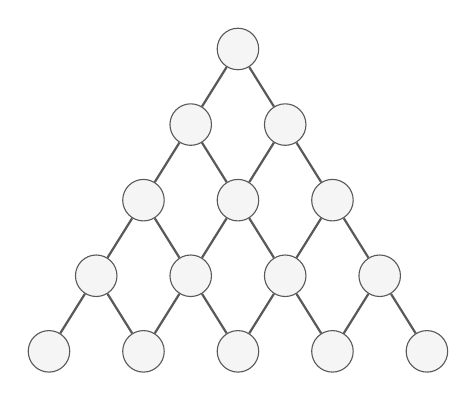
\begin{tikzpicture}[scale=0.8]
            \foreach \n in {0,...,4} {
                \foreach \k in {0,...,\n} {
                    \node[circle, draw=subGray, fill=lightGray, inner sep=2pt, minimum size=1.5em] 
                    (N-\n-\k) at ({\k*1.5 - \n*0.75}, {-\n*1.2}) {};
                }
            }
            \foreach \n in {0,...,3} {
                \foreach \k in {0,...,\n} {
                    \pgfmathtruncatemacro{\nplus}{\n+1}
                    \pgfmathtruncatemacro{\kplus}{\k+1}
                    \draw[subGray, thick] (N-\n-\k) -- (N-\nplus-\k);
                    \draw[subGray, thick] (N-\n-\k) -- (N-\nplus-\kplus);
                }
            }
        \end{tikzpicture}
        
        \vfill
        
        {\large \textbf{Class:} 1年 \underline{\hspace{3em}} 組 \quad \textbf{Name:} \underline{\hspace{12em}}}
        
        \vspace{2cm}
    \end{center}
\end{titlepage}
% =======================================================
% 挿絵 (Art Page)
% =======================================================
\newpage
\thispagestyle{empty}
\vspace*{\fill}

\begin{center}
   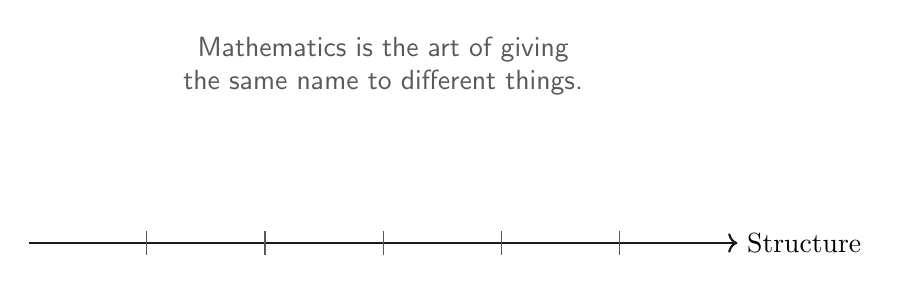
\begin{tikzpicture}[scale=1.5]
       % 二項展開のイメージ
       \draw[thick, mainBlack, ->] (-3,0) -- (3,0);
       \node[right] at (3,0) {Structure};
       
       \foreach \x in {-2, -1, 0, 1, 2} {
            \draw[subGray] (\x, 0.1) -- (\x, -0.1);
       }
       
       \node[align=center, font=\sffamily\color{subGray}] at (0, 1.5) {
           Mathematics is the art of giving\\
           the same name to different things.
       };
   \end{tikzpicture}
\end{center}

\vspace*{\fill}
% =======================================================
% 目次 (Table of Contents)
% =======================================================
\newpage
\thispagestyle{plain}

% 目次の設定
\setcounter{tocdepth}{2}
\tableofcontents

\newpage


% =======================================================
% 第1回
% =======================================================
\setKey{The Rhythm of Expansion}

\section{二項定理:展開の風景}

% --- Page 1 ---
\subsection{Prologue:静寂の中の爆発}

放課後の教室には、西日が長く伸びていた。黒板消しの粉が光の中で舞っている。
私はノートの白いページを前にして、溜息をついた。そこには無機質な計算式が並んでいる。

\[ (a+b)^5 = (a+b)(a+b)(a+b)(a+b)(a+b) \]

\talk{私}{「これを全部展開しろなんて、正気の沙汰じゃないよ。計算ミスをする自信しかない」}

\talk{友人}{「あれ? まだやってたの? ひたすら分配法則でかければいいじゃん。根性、根性」}

部活帰りの友人が、鞄を肩にかけたまま私のノートを覗き込む。彼女は感覚派で、面倒な計算もスポーツのようにこなすが、私はそうはいかない。

\talk{私}{「根性論は嫌いなんだよ。もっとこう、スマートな方法はないのかな」}

\talk{先生}{「おや、良い不満ですね」}

準備室から戻ってきた先生が、チョーク箱を片手に微笑んだ。

\talk{先生}{「『面倒くさい』という感情は、数学において最も重要な才能の一つです。面倒だからこそ、人は法則を探し、構造を見つけようとするのですから」}

先生は黒板に向かうと、静かにチョークを走らせた。

\talk{先生}{「ただ闇雲に計算するのではなく、展開された『式のリズム』に耳を澄ませてみましょう」}

\newpage
\subsection{Topic 1:パスカルの三角形}

先生は黒板に、係数だけを抜き出したピラミッドを描き始めた。

\begin{center}
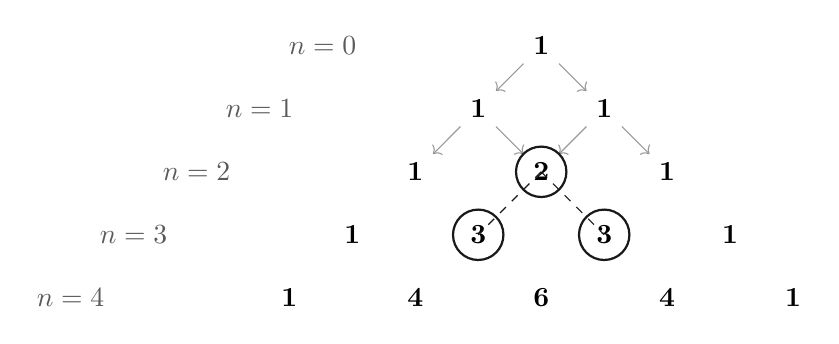
\begin{tikzpicture}[scale=0.8]
    \node (r0) at (0,0) {\textbf{1}};
    \node[left=2cm of r0, subGray] {$n=0$};
    
    \node (r1a) at (-1,-1) {\textbf{1}}; \node (r1b) at (1,-1) {\textbf{1}};
    \node[left=2cm of r1a, subGray] {$n=1$};
    
    \node (r2a) at (-2,-2) {\textbf{1}}; \node (r2b) at (0,-2) {\textbf{2}}; \node (r2c) at (2,-2) {\textbf{1}};
    \node[left=2cm of r2a, subGray] {$n=2$};
    
    \node (r3a) at (-3,-3) {\textbf{1}}; \node (r3b) at (-1,-3) {\textbf{3}}; \node (r3c) at (1,-3) {\textbf{3}}; \node (r3d) at (3,-3) {\textbf{1}};
    \node[left=2cm of r3a, subGray] {$n=3$};
    
    \node (r4a) at (-4,-4) {\textbf{1}}; \node (r4b) at (-2,-4) {\textbf{4}}; \node (r4c) at (0,-4) {\textbf{6}}; \node (r4d) at (2,-4) {\textbf{4}}; \node (r4e) at (4,-4) {\textbf{1}};
    \node[left=2cm of r4a, subGray] {$n=4$};

    % Arrows
    \draw[->, borderGray] (r0) -- (r1a); \draw[->, borderGray] (r0) -- (r1b);
    \draw[->, borderGray] (r1a) -- (r2a); \draw[->, borderGray] (r1a) -- (r2b); \draw[->, borderGray] (r1b) -- (r2b); \draw[->, borderGray] (r1b) -- (r2c);
    
    % Focus circle
    \draw[mainBlack, thick] (0,-2) circle (0.4cm);
    \draw[mainBlack, thick] (-1,-3) circle (0.4cm);
    \draw[mainBlack, thick] (1,-3) circle (0.4cm);
    \draw[dashed, mainBlack] (0,-2) -- (-1,-3);
    \draw[dashed, mainBlack] (0,-2) -- (1,-3);
\end{tikzpicture}
\end{center}

\talk{友人}{「あ、これ知ってる! 上の2つを足すと下の数になるやつだよね? $1+2=3$、みたいな」}

\talk{先生}{「その通り。これを\textbf{パスカルの三角形}と呼びます。$(a+b)^n$ を展開したときの係数は、実はこの三角形の数字と完全に一致するのです」}

\talk{私}{「本当だ……。$n=2$ のときは $1, 2, 1$ だから $a^2 + 2ab + b^2$。$n=3$ なら $1, 3, 3, 1$ だから $a^3 + 3a^2b + 3ab^2 + b^3$ になってる」}

\talk{先生}{「では、$n=4$ のときはどうなりますか?」}

私は三角形の続きを指でなぞる。$1, 3, 3, 1$ の下は、$1, (1+3), (3+3), (3+1), 1$。つまり、$1, 4, 6, 4, 1$ だ。

\talk{私}{「$(a+b)^4 = a^4 + 4a^3b + 6a^2b^2 + 4ab^3 + b^4$……計算しなくても係数がわかる!」}

\talk{先生}{「素晴らしい。しかし、ここで満足してはいけません。なぜ『上の2つを足すと下の数になる』のでしょうか? その\textbf{理由}を言語化できて初めて、我々は構造を理解したと言えます」}

\newpage

\subsection{Topic 2:二項定理の正体}

先生は $(a+b)^3$ を例に挙げ、式を分解して見せた。

\begin{NoteBox}
    $(a+b)^3$ とは、3つの袋 $(a+b), (a+b), (a+b)$ から、それぞれ $a$ か $b$ のどちらかを取り出して掛け合わせるゲームである。
    \begin{itemize}
        \item すべて $a$ を選ぶ $\rightarrow$ $aaa = a^3$ (通り方は1通り)
        \item $b$ を1個だけ選ぶ $\rightarrow$ $aab, aba, baa$ (通り方は3通り $\rightarrow$ $3a^2b$)
        \item $b$ を2個選ぶ $\rightarrow$ $abb, bab, bba$ (通り方は3通り $\rightarrow$ $3ab^2$)
        \item $b$ を3個選ぶ $\rightarrow$ $bbb = b^3$ (通り方は1通り)
    \end{itemize}
\end{NoteBox}

\talk{私}{「なるほど……。展開係数っていうのは、つまり『選び方の数』なんですね」}

\talk{先生}{「そうです。$n$ 個のカッコの中から、$r$ 個の $b$ を選ぶ(残りは自動的に $a$ になる)。その選び方の総数は、数学Aで学んだ\textbf{コンビネーション(組合せ)}で表せますね」}

\begin{SolidBox}
    \textbf{定理:二項定理 (Binomial Theorem)}
    
    $(a+b)^n$ の展開式は以下のようになる。
    \[ (a+b)^n = {}_n \mathrm{C}_0 a^n + {}_n \mathrm{C}_1 a^{n-1}b + \cdots + {}_n \mathrm{C}_r a^{n-r}b^r + \cdots + {}_n \mathrm{C}_n b^n \]
    
    シグマ記号を用いて短く書くと:
    \[ (a+b)^n = \sum_{r=0}^n {}_n \mathrm{C}_r a^{n-r}b^r \]
    
    特に、\textbf{一般項} は ${}_n \mathrm{C}_r a^{n-r}b^r$ である。
\end{SolidBox}

\talk{友人}{「うわ、シグマが出ると急に難しそうに見える……。要するに、$b$ を何個選ぶかで係数が決まるってこと?」}

\talk{先生}{「その感覚で十分です。${}_n \mathrm{C}_r$ は『$n$ 個の中から $r$ 個を選ぶ』記号。パスカルの三角形の数字は、まさにこの ${}_n \mathrm{C}_r$ の値そのものなのです」}

\subsection{Topic 3:特定の項を狙い撃つ}

\talk{先生}{「では、この武器を使って実践的な問題を解いてみましょう。展開式すべてを書く必要はありません。『欲しい項』だけをピンポイントで抜き出すのです」}

\begin{NoteBox}
    \textbf{例題} \\
    $(2x - 1)^6$ の展開式における、$x^4$ の項の係数を求めよ。
\end{NoteBox}

\talk{私}{「ええと、全部で6乗だから、カッコは6個ある。その中から $x$ を4個作りたい」}

\talk{先生}{「構造が見えてきましたね。$2x$ を4回、残りの $(-1)$ を2回選べばよいのです。一般項の式に当てはめてみましょう」}

\begin{align*}
    {}_6 \mathrm{C}_2 \cdot (2x)^4 \cdot (-1)^2 &= 15 \cdot 16x^4 \cdot 1 \\
    &= 240x^4
\end{align*}

\talk{友人}{「あ、そっか! $r$ は $b$ 側の個数だから、この場合は $(-1)$ を2個選ぶってことね。だから ${}_6 \mathrm{C}_2$ なんだ」}

\talk{私}{「${}_6 \mathrm{C}_4$ でも値は同じだけど、計算は小さい数の方が楽だね」}

\talk{先生}{「正解です。係数は $240$。もしこれを愚直に展開していたら、途中で符号ミスをしていたかもしれませんね。『計算しないための計算』、それが定理の力です」}

\newpage
\subsection{Epilogue:数の織物}

黒板には、パスカルの三角形と二項定理の式が美しく並んでいる。
最初は単なる数字の羅列に見えた展開式が、今は「組合せ」という糸で織られた織物のように見えた。

\talk{先生}{「数学の世界では、一見無関係に見えるものが、深いところで繋がっています。展開公式と場合の数。別々に習ったはずの二つが、ここで握手をしている。美しいと思いませんか?」}

\talk{私}{「はい。……ちょっとだけ、感動しました。面倒くさい計算の裏に、こんなルールがあったなんて」}

\talk{友人}{「ま、私はパスカルの三角形を書く方が好きかな。足し算だけで済むし!」}

友人が笑い、先生も目を細める。
教室の外はもう薄暗い。しかし私の手元のノートは、先ほどよりも少しだけ明るく見えた。

だが、物語はここで終わらない。
数の世界には、まだ「割り算」という大きな壁が残っている。

\vspace{2em}
\begin{center}
    \small \itshape To be continued in Lecture 2...
\end{center}

% =======================================================
% 第2回
% =======================================================
\newpage
\setKey{The Two Faces of Equals}

\section{整式の割り算と恒等式:等号の向こう側}

% --- Page 1 ---
\subsection{Prologue:割り切れない想い}

次の日の数学の時間、私は再び絶望していた。黒板には、小学校以来見ることのなかった「筆算」の記号が、しかし今度は $x$ まみれになって鎮座している。

\[
\renewcommand{\arraystretch}{1.2}
\setlength\arraycolsep{1pt}
\begin{array}{r@{\,}l}
 x^2 - x - 3 \\
\cline{2-2}
x-3 \big) \ \overline{x^3 -4x^2 \phantom{+0x} +5 }\\
 x^3 -3x^2\quad\quad\quad~~ \\
\cline{2-2}
 \phantom{x^3} -x^2 \phantom{+0x}\quad~~~ \\
 \phantom{x^3} -x^2 +3x \quad ~~\\
\cline{2-2}
 \phantom{x^3 -x^2} -3x +5 \\
 \phantom{x^3 -x^2} -3x +9 \\
\cline{2-2}
 \phantom{x^3 -x^2 -3x} -4
\end{array}
\]

\talk{私}{「多項式の割り算……。数式を筆算で割るなんて、見た目がグロテスクすぎませんか」}

\talk{友人}{「えー、そう? パズルみたいで結構好きだけどな。上から順番に消していくだけでしょ?」}

友人はシャーペンを軽快に動かし、サクサクと商を求めている。彼女のノートには、整然とした筆算が並んでいた。

\talk{先生}{「『見た目』に惑わされてはいけません。この筆算が示しているのは、整数の割り算と全く同じ\textbf{『構造』}なのですから」}

先生は黒板の隅に、小さく $13 \div 4$ の筆算を書いた。

\talk{先生}{「$13$ を $4$ で割ると、商は $3$ で余りは $1$。これを式で書くとどうなりますか?」}

\talk{私}{「$13 = 4 \times 3 + 1$ です」}

\talk{先生}{「その通り。では、整式でも全く同じことをしてみましょう」}

\subsection{Topic 1:割り算の原理}

先生は黒板の筆算を指し示し、一つの等式を書き下した。

\begin{SolidBox}
    \textbf{定義:整式の割り算 (Division Algorithm)}
    
    ある整式 $A$ を整式 $B$ で割ったときの商を $Q$、余りを $R$ とすると、以下の等式が成り立つ。
    \[ A = BQ + R \]
    ただし、余り $R$ の次数は、割る式 $B$ の次数より低い。
    (割り切れるときは $R=0$)
\end{SolidBox}

\talk{先生}{「$A$ が元の式、$B$ が割る式、$Q$ が商、$R$ が余り。英語の Quotient(商)と Remainder(余り)の頭文字です」}

\talk{私}{「つまり、さっきの筆算は $(x^3 - 4x^2 + 5) = (x-3)(x^2 - x - 3) - 4$ という等式を作っていただけなんですね」}

\talk{先生}{「その『だけ』が重要なのです。複雑に見える $3$ 次式を、$1$ 次式と $2$ 次式の積、そして小さな余りに分解した。これは式の構造を解析する第一歩です」}

\subsection{Topic 2:恒等式という鏡}

\talk{友人}{「ねえ先生、この $A=BQ+R$ って式は、方程式なの? それともただの計算式?」}

友人の何気ない質問に、先生の目が光った。

\talk{先生}{「良い質問です。君たちはこれまで、$\boldsymbol{=}$(イコール)という記号を無造作に使ってきました。しかし、数学における『等しい』には、実は二つの全く異なる意味があるのです」}

先生は黒板の左右に二つの式を書いた。

\begin{center}
    \begin{minipage}{0.45\textwidth}
        \centering
        \textbf{方程式 (Equation)}
        \[ 2x - 4 = 0 \]
        「$x=2$ のとき\textbf{だけ}成り立つ」\\
        (未知数を探すための式)
    \end{minipage}
    \hfill
    \begin{minipage}{0.45\textwidth}
        \centering
        \textbf{恒等式 (Identity)}
        \[ (x+1)^2 = x^2+2x+1 \]
        「\textbf{どんな} $x$ でも成り立つ」\\
        (式の変形そのもの)
    \end{minipage}
\end{center}

\talk{私}{「言われてみれば……。因数分解の公式とかは、右辺と左辺が常に同じ意味ですよね」}

\talk{先生}{「そうです。そして先ほどの割り算の式 $A=BQ+R$ も、\textbf{恒等式}です。どんな $x$ を代入しても、左辺と右辺は必ず一致します。これが恒等式の強みなのです」}

\begin{NoteBox}
    \textbf{恒等式の性質(係数比較法)}
    
    両辺が同じ形ならば、それぞれの係数は等しい。
    \[ ax^2+bx+c = 2x^2+3x-1 \quad \Longrightarrow \quad a=2, \ b=3, \ c=-1 \]
    
    当たり前に見えるが、「構造が同じなら中身も同じ」という強力な論理である。
\end{NoteBox}

\subsection{Topic 3:分数を「分ける」魔法}

\talk{先生}{「恒等式の考え方を使うと、複雑な分数をバラバラに分解することもできます。これを\textbf{部分分数分解}と呼びます」}

先生は不思議な等式を板書した。

\[ \frac{1}{x(x+1)} = \frac{1}{x} - \frac{1}{x+1} \]

\talk{友人}{「うわ、右辺を通分したら……あ、本当だ! 分子の $1$ に戻る!」}

\begin{align*}
    \text{右辺} &= \frac{(x+1) - x}{x(x+1)} = \frac{1}{x(x+1)}
\end{align*}

\talk{先生}{「分母が積の形になっているとき、それを引き算の形に分解できるのです。今はまだ『ふーん』と思うだけかもしれませんが、将来、数列の和を求めたり、積分(面積計算)をしたりするときに、この変形が劇的な効果を発揮します」}

\talk{私}{「『困難は分割せよ』ってやつですか?」}

\talk{先生}{「デカルトの言葉ですね。その通り。大きな塊のままでは扱いにくい式も、小さく分ければ御しやすくなる。数学も人生も同じです」}

\subsection{Epilogue:虚数への入り口}

筆算、恒等式、部分分数分解。
今日の授業は「式の変形」に終始した。しかし、それは単なる式変形ではなく、「式が持つ本来の姿」を浮き彫りにする作業だったように感じる。

\talk{先生}{「さて。ここまでは『実数』の世界で式をいじくり回してきました。しかし、君たちは覚えているでしょうか? 2次方程式の解の公式において、ルートの中身がマイナスになったときのあの絶望を」}

\talk{友人}{「あー、『解なし』ってやつね。あれ書くとテストが終わった気がしてスッキリするんだよね」}

\talk{先生}{「本当に『なし』で終わらせていいのでしょうか? もし、2乗してマイナスになる数が存在したら……この割り算や恒等式の世界は、どう広がると思いますか?」}

先生は悪戯っぽく笑い、チョークを置いた。

\talk{先生}{「次回、我々は禁断の領域に足を踏み入れます。その数の名は、イマジナリー・ナンバー」}

教室の窓の外、夕焼けが少しだけ紫がかって見えた。
常識が崩れる予感がした。

\vspace{2em}
\begin{center}
    \small \itshape To be continued in Lecture 3...
\end{center}

% =======================================================
% 第3回
% =======================================================
\newpage
\setKey{The Imaginary Gateway}

\section{複素数の導入:禁じられた数}

% --- Page 1 ---
\subsection{Prologue:行き止まりの壁}

「二乗して $-1$ になる数は?」
先生のその問いかけに、教室は沈黙した。

\talk{私}{「ありません。実数の二乗は必ずプラスか $0$ になる。それが『実数』の定義みたいなものじゃないですか」}

\talk{先生}{「その通り。数直線上に住んでいる限り、この問いは『解なし』という行き止まりです。しかし……もし、この壁の向こう側に行けるとしたら?」}

先生は黒板に大きな扉の絵を描き、その中央に $i$ という文字を記した。

\talk{先生}{「人間は、自然数から整数へ、整数から有理数へ、そして実数へと、必要に応じて『数』の概念を拡張してきました。ならば、もう一歩踏み出しても罰は当たらないでしょう。ようこそ、\textbf{New Game} の世界へ」}

\subsection{Topic 1:虚数単位 $i$ の誕生}

先生は厳かに宣言した。

\begin{SolidBox}
    \textbf{定義:虚数単位 (Imaginary Unit)}
    
    2乗して $-1$ になる新しい数を $\bm{i}$ で表す。
    \[ i^2 = -1 \]
\end{SolidBox}

% Ref: [cite: 63]

\talk{友人}{「$i$ って、imaginary(想像上の)の頭文字? なんか中二病っぽくてカッコいいね」}

\talk{先生}{「デカルトが『想像上の数』と呼んだのが始まりですが、今やこの数は電気工学や量子力学になくてはならない『現実的』な道具です。存在するかどうかではなく、\textbf{そういうルールを定めたら計算がどうなるか}を楽しむのが数学ですよ」}

\subsection{Topic 2:複素数というハイブリッド}

\talk{先生}{「さて、この新しい住人 $i$ を、従来の実数と組み合わせると、\textbf{複素数 (Complex Number)} という新しい数が生まれます」}

\[ \bm{a + bi} \quad (a, b \text{ は実数}) \]

% Ref: [cite: 64]

\talk{先生}{「$a$ を\textbf{実部}、$b$ を\textbf{虚部}と呼びます。例えば $3+2i$ のような形です」}

\talk{私}{「$3$ と $2i$ は足して $5i$ とかにはならないんですか?」}

\talk{先生}{「なりません。水と油のように、実部と虚部は混ざり合いません。混ざらないからこそ、等しいかどうかの判定も厳密になります」}

\begin{NoteBox}
    \textbf{複素数の相等}
    
    \[ a+bi = c+di \quad \iff \quad a=c \ \text{かつ} \ b=d \]
    
    特に、
    \[ a+bi = 0 \quad \iff \quad a=0 \ \text{かつ} \ b=0 \]
\end{NoteBox}

% Ref: [cite: 67, 68]

\talk{友人}{「つまり、実部同士、虚部同士を別々に比べればいいんだね。連立方程式みたい」}

\talk{先生}{「その感覚です。$i$ というタグがついているものと、ついていないものを分けて管理するのです」}

\subsection{Topic 3:計算のルール}

\talk{先生}{「計算自体は、文字式 $x$ を含む計算とほとんど同じです。たった一つ、\textbf{魔法のルール}を除いては」}

\talk{私}{「$i^2$ が出てきたら $-1$ に変える、ですね」}

\talk{先生}{「そうです。試しに掛け算をやってみましょう」}

\begin{align*}
    (2+i)(3-2i) &= 2(3-2i) + i(3-2i) \\
    &= 6 - 4i + 3i - 2i^2 \quad (\leftarrow \text{普通の展開}) \\
    &= 6 - i - 2(\bm{-1}) \quad (\leftarrow \text{魔法発動!}) \\
    &= 6 - i + 2 \\
    &= 8 - i
\end{align*}

% Ref: [cite: 72]

\talk{友人}{「おー! $i^2$ が実数に戻るから、最後に実部同士を合体できるんだ。なんかパズルみたいで楽しいかも」}

\talk{先生}{「この『実数に戻る』という性質が、複素数の世界と実数の世界を繋ぐ架け橋になります」}

\subsection{Topic 4:ルートの中のマイナス}

授業の最後に、先生は注意深く黒板の一角を消し、赤いチョークを手に取った。

\talk{先生}{「最後に一つだけ、絶対に踏んではいけない地雷を教えましょう」}

\begin{SolidBox}
    \textbf{負の数の平方根}
    
    $a>0$ のとき、$\sqrt{-a} = \sqrt{a}i$ と定義する。
    
    \vspace{0.5em}
    \textbf{注意:} 計算するときは、\textbf{必ず先に $i$ を外に出すこと!}
\end{SolidBox}

% Ref: [cite: 73, 74]

\talk{先生}{「例えば、$\sqrt{-2} \times \sqrt{-3}$ を計算するとき、中身を掛けて $\sqrt{6}$ としてはいけません」}

\talk{私}{「え、ダメなんですか? $\sqrt{a}\sqrt{b}=\sqrt{ab}$ って習いましたけど」}

\talk{先生}{「それは中身がプラスの時だけのルールです。見てごらんなさい」}

\begin{align*}
    \text{誤} &:\quad \sqrt{-2} \times \sqrt{-3} = \sqrt{(-2)\times(-3)} = \sqrt{6} \\
    \text{正} &:\quad \sqrt{-2} \times \sqrt{-3} = \sqrt{2}i \times \sqrt{3}i = \sqrt{6} \bm{i^2} = -\sqrt{6}
\end{align*}

% Ref: [cite: 75]

\talk{私}{「うわっ、符号が逆になった!」}

\talk{先生}{「$i$ を介さないと、このマイナスの符号を見落としてしまうのです。負の平方根を見たら、反射的に $i$ を外に出す。これを徹底してください」}

\subsection{Epilogue:大小のない世界}

チャイムが鳴り、先生はチョークの粉を払った。

\talk{先生}{「ちなみに、$3+2i$ と $5i$ はどちらが大きいと思いますか?」}

\talk{友人}{「えーっと、$5i$ の方が係数が大きいから……」}

\talk{先生}{「残念ながら、複素数の世界には\textbf{大小関係が存在しません}。大きいも小さいもない。数直線上には乗らない数なのですから」}

私たちは顔を見合わせた。大小がない世界。それは今までの「数」の常識が通用しない、全く新しい荒野だ。

\talk{私}{「先生、この $i$ を使うと、今まで解けなかった方程式が解けるようになるんですか?」}

\talk{先生}{「ええ。次回は、かつて『解なし』と捨てていた二次方程式の残骸を拾いに行きましょう。そこには、美しい『共役』のペアが待っています」}

\vspace{2em}
\begin{center}
    \small \itshape To be continued in Lecture 4...
\end{center}


% =======================================================
% 第4回
% =======================================================
\newpage
\setcounter{section}{3} % 第4回なのでカウンターを3にセット(次は4になる)
\setKey{Twin Souls \& The Discriminant}

\section{共役複素数と判別式:対なる魂と判別の瞳}

% --- Page 1 ---
\subsection{Prologue:割り算という名の浄化}

放課後の補習室。私は黒板に書かれた分数式を睨みつけていた。

\[ \frac{1+2i}{3+i} \]

\talk{私}{「足し算と引き算は実部・虚部を分けるだけ。掛け算は $i^2=-1$ にすればいい。でも先生、\textbf{割り算}ってどうするんですか? $3+i$ で割るって、イメージが湧きません」}

\talk{友人}{「約分……はできないしね。分母に $i$ があるとなんか気持ち悪い」}

\talk{先生}{「その『気持ち悪い』という感覚は正しい。数学では、分母にルートがあるのを嫌って『有理化』しましたよね? 同じように、分母に $i$ があるのも解消したいのです」}

先生はチョークを手に取り、分母の $3+i$ の隣に、ある式を書き添えた。

\talk{先生}{「毒をもって毒を制す。$i$ を消し去るためには、相棒が必要なのです」}

\subsection{Topic 1:共役(きょうやく)な複素数}

先生が書き足したのは、$3\mathbf{-}i$ だった。

\begin{SolidBox}
    \textbf{定義:共役な複素数 (Conjugate Complex Numbers)}
    
    複素数 $z = a+bi$ に対して、虚部の符号を変えた $a-bi$ を、
    $z$ の\textbf{共役な複素数}といい、記号 $\bar{z}$ で表す。
    \[ z = a+bi \quad \Longrightarrow \quad \bar{z} = a-bi \]
\end{SolidBox}

\talk{友人}{「プラスをマイナスにするだけ? 簡単じゃん」}

\talk{先生}{「単純ですが、効果は絶大です。このペアは非常に仲が良く、\textbf{足しても掛けても実数に戻る}という性質を持っています」}

先生は実際に計算してみせた。

\begin{align*}
    \text{和} &:\quad (a+bi) + (a-bi) = 2a \\
    \text{積} &:\quad (a+bi)(a-bi) = a^2 - (bi)^2 = a^2 - b^2(-1) = \mathbf{a^2+b^2}
\end{align*}

\talk{私}{「あ! 積の公式 $(x+y)(x-y)=x^2-y^2$ が使えるんですね。$i^2$ が $-1$ だから、結果的に $a^2+b^2$ になって、$i$ が消える!」}

\talk{先生}{「そうです。これを利用すれば、分母の実数化が可能になります」}

\begin{NoteBox}
    \textbf{例:分母の実数化}
    
    分母・分子に、分母の共役複素数 $3-i$ を掛ける。
    \begin{align*}
        \frac{1+2i}{3+i} &= \frac{(1+2i)(3-i)}{(3+i)(3-i)} \\
        &= \frac{3-i+6i-2i^2}{3^2+1^2} = \frac{5+5i}{10} = \frac{1}{2} + \frac{1}{2}i
    \end{align*}
\end{NoteBox}

\newpage

% --- Page 2 ---
\subsection{Topic 2:解の公式、再訪}

\talk{先生}{「さて、複素数の計算に慣れたところで、我々の本来の目的である\textbf{2次方程式}に戻りましょう」}

先生は黒板の隅にあった「解なし」の文字を消し、新たな方程式を書いた。

\[ x^2 + x + 1 = 0 \]

\talk{私}{「これ、解の公式を使うとルートの中がマイナスになりますよ。$D = 1^2 - 4 = -3$ だから……」}

\talk{先生}{「これまではそこで『解なし』と諦めていました。しかし、今の君たちには $i$ という武器がある。進みなさい」}

私は恐る恐るノートにペンを走らせる。

\begin{align*}
    x &= \frac{-1 \pm \sqrt{1^2 - 4 \cdot 1 \cdot 1}}{2} \\
      &= \frac{-1 \pm \sqrt{-3}}{2}
\end{align*}

\talk{私}{「……ここで、$\sqrt{-3} = \sqrt{3}i$ と書き換えればいいんですね?」}

\[ x = \frac{-1 \pm \sqrt{3}i}{2} \]

\talk{先生}{「正解です。かつて『解なし』だった方程式は、複素数の世界では\textbf{『異なる2つの虚数解』}を持つのです」}

\talk{友人}{「虚数解……なんか響きがカッコいい。でもこれ、現実に意味あるの?」}

\talk{先生}{「意味は大ありです。この解をよく見てください。$\frac{-1+\sqrt{3}i}{2}$ と $\frac{-1-\sqrt{3}i}{2}$……この二つの関係は?」}

\talk{私}{「あ、虚部のプラスマイナスが違うだけ……\textbf{共役}になってます!」}

\talk{先生}{「その通り。実数係数の2次方程式が虚数解を持つとき、それらは必ず\textbf{共役な複素数のペア}で現れます。独りぼっちの虚数解は存在しないのです」}

\newpage

% --- Page 3 ---
\subsection{Topic 3:判別式という検問所}

先生は大きな3つのグラフを黒板に描き始めた。

\talk{先生}{「ルートの中身 $b^2-4ac$、これを\textbf{判別式 $D$}と呼びます。この符号は、単に計算の途中経過ではなく、\textbf{グラフの形そのもの}を支配しています」}

\begin{SolidBox}
    \textbf{定理:判別式 (Discriminant)}
    
    2次方程式 $ax^2+bx+c=0$ の解の種類は、判別式 $D = b^2 - 4ac$ の符号で決まる。
\end{SolidBox}

\vspace{1em}
\begin{center}
\begin{tikzpicture}[scale=0.9, >=stealth]
    % D > 0
    \begin{scope}[xshift=-5cm]
        \draw[->] (-2,0) -- (2,0) node[right] {$x$};
        \draw[thick, mainBlack] plot[domain=-1.5:1.5] (\x, {\x*\x - 1});
        \node[above] at (0,1.5) {\large $\mathbf{D > 0}$};
        \fill[subGray] (-1,0) circle (2pt);
        \fill[subGray] (1,0) circle (2pt);
        \node[below, align=center, font=\small] at (0,-1.5) {\textbf{異なる2つの実数解}\\(交点2つ)};
    \end{scope}

    % D = 0
    \begin{scope}[xshift=0cm]
        \draw[->] (-2,0) -- (2,0) node[right] {$x$};
        \draw[thick, mainBlack] plot[domain=-1.5:1.5] (\x, {\x*\x});
        \node[above] at (0,1.5) {\large $\mathbf{D = 0}$};
        \fill[subGray] (0,0) circle (2pt);
        \node[below, align=center, font=\small] at (0,-1.5) {\textbf{ただ1つの実数解}\\(重解・接する)};
    \end{scope}

    % D < 0
    \begin{scope}[xshift=5cm]
        \draw[->] (-2,0) -- (2,0) node[right] {$x$};
        \draw[thick, mainBlack] plot[domain=-1.5:1.5] (\x, {\x*\x + 0.5});
        \node[above] at (0,1.5) {\large $\mathbf{D < 0}$};
        % 交点なし
        \node[below, align=center, font=\small] at (0,-1.5) {\textbf{異なる2つの虚数解}\\(交点なし)};
    \end{scope}
\end{tikzpicture}
\end{center}

\talk{先生}{「$D<0$ は、ゲームオーバーのサインではなく、『ここから先は虚数世界』という標識だったのです」}

\talk{友人}{「実数解ルートか、虚数解ルートか、分岐点で決まるって感じだね」}

\subsection{Epilogue:見えない交点}

\talk{私}{「でも先生、グラフで考えると不思議です。$D<0$ のときって、放物線は $x$軸と交わらないですよね(浮いている)。交点がないのに、解があるってどういうことですか?」}

私は空中に放物線を描いてみせる。

\talk{先生}{「鋭いですね。確かに、我々が見ている\textbf{実平面(xy平面)}上には交点はありません。しかし、次元を拡張した『複素空間』では、グラフは確かに交わっているのです」}

先生は黒板に描いた放物線のグラフを見つめ、静かに言った。

\talk{先生}{「目に見えるものだけが真実とは限りません。方程式は、目に見えない場所でも解を持っている。……さて、解が手に入ったら、次はそれを使って遊びたくなりませんか?」}

\talk{私}{「遊ぶ?」}

\talk{先生}{「解を足したり引いたりして、元の係数との関係を探るのです。次回は、解と係数の美しい関係性についてお話ししましょう」}

\vspace{2em}
\begin{center}
    \small \itshape To be continued in Lecture 5...
\end{center}

% =======================================================
% 第5回
% =======================================================
\newpage
\setcounter{section}{4} % 第5回
\setKey{The Dance of Symmetry}

\section{解と係数の関係:対称性のダンス}

% --- Page 1 ---
\subsection{Prologue:究極の手抜き}

「はぁ……」
友人が深い溜息をついた。ノートには、解の公式を使って求めた複雑な解が並んでいる。

\[ x = \frac{3 \pm \sqrt{7}i}{2} \]

\talk{友人}{「ねえ、この解を2つ足して、とか、掛けて、って言われたら地獄じゃない? 分数の足し算も面倒だし、掛け算なんて展開して $i^2$ して……計算ミスする気しかしない」}

\talk{私}{「確かに。でも、入試問題とかでよく見るよね。『$\alpha^2 + \beta^2$ を求めよ』みたいなやつ」}

\talk{先生}{「お困りのようですね。しかし、君たちのその『面倒くさい』という感覚は正しい。賢い数学者は、わざわざ解を求めてから計算したりはしません」}

先生は黒板に $ax^2+bx+c=0$ と書き、チョークを空中に投げ上げた。パチリ、とキャッチする。

\talk{先生}{「解を知らなくても、解の『和』と『積』だけなら、係数を見るだけで分かるのです。それも、一瞬で」}

\subsection{Topic 1:復元という逆転の発想}

先生は少し悪戯っぽい顔をして、黒板に数式を書き始めた。

\talk{先生}{「もし、2次方程式 $ax^2+bx+c=0$ の解が $\alpha, \beta$ だと分かっていたら、この方程式はどう因数分解できますか?」}

\talk{私}{「ええと……解が $\alpha, \beta$ ということは、$(x-\alpha)$ と $(x-\beta)$ を因数に持つはずです」}

\talk{先生}{「その通り。ただし、最高次の係数 $a$ を忘れないでくださいね」}

先生は鮮やかに式変形を展開していく。

\begin{align*}
    ax^2+bx+c &= a(x-\alpha)(x-\beta) \\
              &= a(x^2 - (\alpha+\beta)x + \alpha\beta) \\
              &= a x^2 - a(\alpha+\beta)x + a\alpha\beta
\end{align*}

\talk{先生}{「さあ、元の式と係数を比べてごらんなさい」}

\[
\begin{cases}
    x \text{ の係数}: & b = -a(\alpha+\beta) \\
    \text{定数項}: & c = a\alpha\beta
\end{cases}
\]

\talk{私}{「あ! これを変形すれば……」}

\begin{SolidBox}
    \textbf{定理:解と係数の関係 (Vieta's Formulas)}
    
    2次方程式 $ax^2+bx+c=0$ の2つの解を $\alpha, \beta$ とすると、
    \[ \mathbf{\alpha+\beta = -\frac{b}{a}}, \quad \mathbf{\alpha\beta = \frac{c}{a}} \]
\end{SolidBox}



\talk{友人}{「嘘でしょ? 解の公式であんなに苦労してたのが、分数ポン、で終わり?」}

\talk{先生}{「ええ。和はマイナス・アのブ($-b/a$)、積はアのク($c/a$)。これさえ覚えておけば、解そのものを求める必要はありません」}

\newpage

% --- Page 2 ---
\subsection{Topic 2:対称式の魔法}

\talk{先生}{「さて、ここからが本番です。和 $\alpha+\beta$ と 積 $\alpha\beta$ という2つのパーツを手に入れました。実はこの2つさえあれば、\textbf{対称式}と呼ばれるあらゆる式を作り出すことができます」}

\begin{NoteBox}
    \textbf{対称式とは}
    
    文字 $\alpha, \beta$ を入れ替えても値が変わらない式のこと。
    (例:$\alpha^2+\beta^2$, $\frac{1}{\alpha}+\frac{1}{\beta}$ など)
    
    すべての対称式は、基本対称式 $(\alpha+\beta)$ と $\alpha\beta$ だけで表せる。
\end{NoteBox}



\talk{先生}{「例えば、友人が嫌がっていた $\alpha^2+\beta^2$。これを $(\alpha+\beta)^2$ の形から作ろうとすると、余計なものが出てきますね?」}

\[ (\alpha+\beta)^2 = \alpha^2 + 2\alpha\beta + \beta^2 \]

\talk{私}{「真ん中の $2\alpha\beta$ が邪魔ですね」}

\talk{先生}{「邪魔なら引けばいいのです」}

\[ \mathbf{\alpha^2+\beta^2 = (\alpha+\beta)^2 - 2\alpha\beta} \]

\talk{友人}{「なるほど! ブロック遊びみたい。和の2乗から、積の2倍を引けばいいんだ」}

\talk{先生}{「その通り。同様に、逆数の和も通分すれば……」}

\[ \mathbf{\frac{1}{\alpha} + \frac{1}{\beta} = \frac{\alpha+\beta}{\alpha\beta}} \]

\talk{先生}{「ほら、また和と積だけで表せました。解を直接代入して計算するより、遥かにスマートでしょう?」}

\subsection{Topic 3:方程式を創る}

授業の終盤、先生はさらに問いかけた。

\talk{先生}{「我々は今、方程式から和と積を取り出しました。では逆に、\textbf{和と積から方程式を復元する}ことはできますか?」}

\talk{私}{「ええと、さっきの式の逆をやればいいんですよね」}

\begin{SolidBox}
    \textbf{2数を解とする方程式}
    
    2数 $\alpha, \beta$ を解にもつ2次方程式の一つは、
    \[ x^2 - (\text{和})x + (\text{積}) = 0 \]
    つまり、
    \[ x^2 - (\alpha+\beta)x + \alpha\beta = 0 \]
\end{SolidBox}



\talk{先生}{「例えば、和が $3$、積が $5$ になる2つの数を求めよ、と言われたら?」}

\talk{私}{「$x^2 - 3x + 5 = 0$ を解けばいい!」}

\talk{先生}{「正解です。直接探すのは大変ですが、方程式という『型』に流し込めば、あとは解の公式が仕事をしてくれます」}

\newpage

\subsection{Epilogue:次数の階段へ}

\talk{友人}{「今日はなんか、狐につままれた気分。解いてないのに解のことが分かるなんて」}

\talk{先生}{「それが構造を見るということです。個々の解(具体的な数値)に囚われず、それらが織りなす関係性(係数)を見る。視点を一つ上げたのですよ」}

先生は黒板を消しながら、楽しげに言った。

\talk{先生}{「さて、2次方程式の世界はこれで制覇しました。しかし、君たちの前にはまだ、3次、4次という『高次方程式』の山がそびえています」}

\talk{私}{「3次方程式……解の公式はあるんですか?」}

\talk{先生}{「あります。ありますが、あまりに長すぎて覚える気にはなれないでしょう。そこで次回は、別の武器を用意します。『割り算』と『因数分解』の合わせ技、\textbf{因数定理}です」}

\vspace{2em}
\begin{center}
    \small \itshape To be continued in Lecture 6...
\end{center}

% =======================================================
% 第6回
% =======================================================
\newpage
\setcounter{section}{5} % 第6回
\setKey{The Remainder's Secret}

\section{剰余の定理と因数定理:余りの行方}

% --- Page 1 ---
\subsection{Prologue:割り算をしたくない理由}

「$x^3 - 3x^2 + 4x - 5$ を $x-2$ で割った余りを求めよ」

黒板に書かれた問題を見て、私は反射的に筆算の記号を書き始めた。
$x^3$ を消すために $x^2$ を立てて……引いて……次は $-x$ を立てて……。

\talk{私}{「……面倒くさいです。計算ミスしそうだし、もっと楽に『余り』だけ知る方法はないんですか?」}

\talk{友人}{「横着だなぁ。でも確かに、商はいらないから余りだけ教えて、って時あるよね」}

\talk{先生}{「その横着こそが進化の母です。実は、\textbf{割り算を一切せずに余りだけを透視する方法}があります」}

先生は私のノートの筆算を手で隠し、代わりに元の式 $P(x)$ を指差した。

\talk{先生}{「この式の $x$ に、ある数字を代入するだけです。試しに $2$ を入れてごらんなさい」}

\subsection{Topic 1:剰余の定理}

言われるがままに、$P(x) = x^3 - 3x^2 + 4x - 5$ に $x=2$ を代入してみる。

\begin{align*}
    P(2) &= 2^3 - 3(2^2) + 4(2) - 5 \\
         &= 8 - 12 + 8 - 5 \\
         &= -1
\end{align*}

\talk{私}{「$-1$ になりました」}

\talk{先生}{「では、さっき途中で投げ出した筆算を最後までやってみてください」}

私は渋々計算を続けた。……結果、余りは $-1$。

\talk{私}{「一致した! え、なんでですか?」}

\talk{先生}{「恒等式の魔法です。割り算の式を思い出してください」}

\[ P(x) = (x-k)Q(x) + R \]

\talk{先生}{「この式の $x$ に $k$ を代入すると、どうなりますか?」}

\talk{私}{「$(k-k)$ で……あ! 商 $Q(x)$ の部分が $0$ になって消える!」}

\[ P(k) = 0 \cdot Q(k) + R \quad \Longrightarrow \quad \mathbf{R = P(k)} \]

\talk{先生}{「商 $Q(x)$ がどんなに複雑でも関係ありません。割る式が $0$ になるスイッチを押せば、商もろとも消え去り、余りだけがポロリと落ちてくるのです」}

\begin{SolidBox}
    \textbf{定理:剰余の定理 (Remainder Theorem)}
    
    整式 $P(x)$ を 1次式 $x-k$ で割った余りは、$\mathbf{P(k)}$ に等しい。
    
    \vspace{0.5em}
    \textbf{応用:} $ax+b$ で割った余りは、$P\left(-\frac{b}{a}\right)$ に等しい。
    (割る式が $0$ になる $x$ の値を代入せよ)
\end{SolidBox}



\talk{友人}{「なるほど……。$x+1$ で割るなら $x=-1$ を代入すればいいってことね。これなら暗算でもいけそう」}

\newpage

\subsection{Topic 2:因数定理}

\talk{先生}{「さて、ここからが本題です。もし、代入して計算した結果、\textbf{余りが 0 になったら}どういうことでしょうか?」}

\talk{私}{「割り切れる、ということです」}

\talk{先生}{「割り切れるということは?」}

\talk{私}{「ええと……因数分解できる、ということですか?」}

\talk{先生}{「その通り!」}

先生は大きく頷き、黒板に重要な定理を記した。

\begin{SolidBox}
    \textbf{定理:因数定理 (Factor Theorem)}
    
    整式 $P(x)$ について、
    \[ \mathbf{P(k)=0 \iff P(x) \text{ は } x-k \text{ を因数にもつ}} \]
\end{SolidBox}



\talk{先生}{「これは強力な武器です。どんなに複雑な高次式でも、『代入して $0$ になる数』さえ見つければ、そこから因数分解の糸口が掴めるのですから」}

\newpage

% --- Page 2 ---
\subsection{Topic 3:高次式の因数分解}

先生は3次式 $x^3 - 4x^2 + x + 6$ を黒板に書いた。公式一発では解けない形だ。

\talk{先生}{「演習の時間です。この式に代入して $0$ になる数(解の候補)を探してください。ヒントは\textbf{定数項の約数}です」}

\talk{友人}{「定数項は $6$ だから…… $\pm 1, \pm 2, \pm 3, \pm 6$ のどれか?」}

私たちは手当たり次第に代入を始めた。

\begin{itemize}
    \item $x=1$ のとき: $1 - 4 + 1 + 6 = 4 \neq 0$ (ハズレ)
    \item $x=-1$ のとき: $-1 - 4 - 1 + 6 = 0$ (\textbf{アタリ!})
\end{itemize}

\talk{私}{「先生! $-1$ で $0$ になりました!」}

\talk{先生}{「素晴らしい。ということは、この式は必ず $(x+1)$ を因数に持ちます。あとは実際に割ってみれば……」}

私は見つかった $(x+1)$ で筆算を行った。今度は商が必要だからだ。

\[ (x^3 - 4x^2 + x + 6) \div (x+1) = x^2 - 5x + 6 \]

\talk{先生}{「残りの部分は2次式になりましたね。これなら君たちにも解けるはずです」}

\talk{友人}{「$x^2 - 5x + 6$ は $(x-2)(x-3)$ に分解できる! ということは……」}

\[ x^3 - 4x^2 + x + 6 = (x+1)(x-2)(x-3) \]

\talk{私}{「できた……。3次式がバラバラになった」}

\newpage

\subsection{Epilogue:次数の壁を越えて}

\talk{先生}{「因数定理を使えば、3次以上の方程式でも、1つ解を見つけるだけで次数を下げることができます。次数が下がれば、あとは我々の知っている土俵(2次方程式)に持ち込める」}

先生は満足げにチョークを置いた。

\talk{先生}{「次回は、いよいよこれを使って高次方程式を解きまくります。ただし、中には実数の範囲では因数分解しきれない、厄介な相手もいますがね」}

\talk{友人}{「厄介な相手?」}

\talk{先生}{「ええ。例えば $x^3=1$ を解くと、虚数の世界への扉が再び開きます。そこには $\omega$(オメガ)という不思議な数が住んでいるのです」}

\vspace{2em}
\begin{center}
    \small \itshape To be continued in Lecture 7...
\end{center}

% =======================================================
% 第7回
% =======================================================
\newpage
\setcounter{section}{6} % 第7回
\setKey{Divide and Conquer}

\section{高次方程式:次数の呪縛を解く}

% --- Page 1 ---
\subsection{Prologue:公式の不在}

黒板には3次方程式が静かに佇んでいた。

\[ x^3 - 4x^2 + 8x - 5 = 0 \]

\talk{私}{「先生、2次方程式には『解の公式』という万能の鍵がありましたが……3次方程式にも同じような公式があるのでしょうか?」}

\talk{先生}{「存在はします。カルダノの公式などが有名ですが、実用するにはあまりに複雑すぎます。高校数学の範疇では、公式に頼ることは得策ではありません」}

\talk{友人}{「えっ、じゃあどうやって解くの? 勘で当てるとか?」}

\talk{先生}{「『勘』ではありません。『洞察』です。どんなに高次の方程式であっても、基本戦略は一つしかありません。すなわち、\textbf{次数を下げること}。困難を分割し、我々が扱える1次や2次の世界へと引きずり下ろすのです」}

\subsection{Topic 1:因数分解というメス}

先生は黒板の方程式を指し示した。

\talk{先生}{「前回学んだ『因数定理』を思い出してください。この式 $P(x)$ を $0$ にする $x$ の値(解の候補)を見つけることが、すべての始まりです」}

\talk{私}{「定数項 $-5$ の約数を試すんでしたね。$1, -1, 5, -5$……まずは $1$ を代入してみます」}

\[ P(1) = 1 - 4 + 8 - 5 = 0 \]


\talk{私}{「あ、$0$ になりました! ということは、この式は $(x-1)$ を因数に持ちます」} [cite: 14]

\talk{先生}{「よろしい。一つ解が見つかれば、3次方程式は『1次式』と『2次式』の積に分解できます。さあ、割り算を行いなさい」}

私はノートの隅で筆算を始めた。

\[
\renewcommand{\arraystretch}{1.2}
\setlength\arraycolsep{1pt}
\begin{array}{r@{\,}l}
 x^2 - 3x + 5 \\
\cline{2-2}
x-1 \big) \ \overline{x^3 -4x^2 +8x -5} \\
 x^3 -\phantom{4}x^2 \\
\cline{2-2}
 \phantom{x^3} -3x^2 +8x \\
 \phantom{x^3} -3x^2 +3x \\
\cline{2-2}
 \phantom{x^3 -3x^2} 5x -5 \\
 \phantom{x^3 -3x^2} 5x -5 \\
\cline{2-2}
 \phantom{x^3 -3x^2 +5x} 0
\end{array}
\]


\talk{先生}{「筆算は、式変形のプロセスを可視化する優れた手法です。組立除法というテクニックもありますが、構造を理解するまでは堂々と筆算を使うことを推奨します」}


割り算の結果、方程式は次のように変形された。

\[ (x-1)(x^2 - 3x + 5) = 0 \]


\talk{先生}{「これで勝負ありです。あとは、それぞれの因数が $0$ になる瞬間を探ればよい」} [cite: 15]

\begin{itemize}
    \item $x-1=0 \implies x=1$
    \item $x^2-3x+5=0 \implies$ 解の公式より $x = \frac{3 \pm \sqrt{9-20}}{2} = \frac{3 \pm \sqrt{11}i}{2}$
\end{itemize}

\talk{友人}{「うわ、また虚数が出てきた。でも、これで『解けた』ってことにしていいの?」}

\talk{先生}{「もちろんです。実数解が1つ、虚数解が2つ。合わせて3つの解。3次方程式の物語はこれで完結です」}
\newpage

\begin{SolidBox}
    \textbf{高次方程式の解法アルゴリズム}
    \begin{enumerate}
        \item \textbf{解の探索}:因数定理 $P(k)=0$ となる $k$ を見つける。
        \item \textbf{次元の縮小}:$P(x)$ を $(x-k)$ で割り算し、次数を下げる。
        \item \textbf{各個撃破}:分解された方程式をそれぞれ解く。
    \end{enumerate}
    どんなに次数が高くても、この手順を繰り返すだけです。
\end{SolidBox}


\newpage

% --- Page 2 ---
\subsection{Topic 2:複二次式への視点}

\talk{先生}{「次は、少し特殊な形を見てみましょう。一見すると4次方程式ですが、構造をよく観察してください」}


\[ x^4 - 3x^2 - 4 = 0 \] 


\talk{私}{「$x^4$ と $x^2$ しかありません。奇数乗の項がないですね」}

\talk{先生}{「この形を\textbf{複二次式}と呼びます。この式において、$x$ は本当に主役でしょうか? 真の主役は別にいるように見えませんか?」}

\talk{友人}{「真の主役……? あ、$x^2$ をひとかたまりで見ればいいってこと?」}


\talk{先生}{「その通り。$x^2 = X$ と置き換えてごらんなさい。世界がシンプルになります」} 


$X = x^2$ とおくと、方程式は $X^2 - 3X - 4 = 0$ となる。これなら中学生でも解ける因数分解だ。

\[ (X-4)(X+1) = 0 \]

\talk{私}{「つまり、$X=4$ または $X=-1$ ですね」}

\talk{先生}{「しかし、そこで安心してはいけません。我々が求めているのは $X$ ではなく $x$ です。借りたものは返さねばなりません」}

\begin{itemize}
    \item $X=4$ のとき: $x^2 = 4 \implies x = \pm 2$
    \item $X=-1$ のとき: $x^2 = -1 \implies x = \pm i$
\end{itemize}

\talk{友人}{「おー、解が4つ出た! さすが4次方程式」}

\talk{先生}{「置き換えによって視点を変えることで、既知の問題へと帰着させる。数学における最もエレガントな手法の一つです」}
\newpage

\subsection{Epilogue:解の在処}

黒板には、計算されたばかりの解たちが並んでいる。実数、虚数、それらが混ざり合いながら方程式を満たしている。

\talk{先生}{「諸君、方程式を解くという行為は、霧の中に隠された山頂を探すようなものです。公式という地図がない場所では、因数定理というコンパスと、筆算という自分の足だけが頼りです」}

先生は窓の外、遠くの稜線を眺めながら言った。

\talk{先生}{「しかし、時にはコンパスさえ効かない深い森もあります。グラフと方程式が複雑に絡み合う領域……次回は、数式と図形が交差する場所、『グラフと方程式』の関係性について思索を深めましょう」}

\vspace{2em}
\begin{center}
    \small \itshape To be continued in Lecture 8...
\end{center}

% =======================================================
% 第8回
% =======================================================
\newpage
\setcounter{section}{7} % 第8回
\setKey{Where Equations Meet Geometry}

\section{方程式とグラフ:交錯する運命}

% --- Page 1 ---
\subsection{Prologue:デカルトの眼鏡}

先生は黒板に、数式とグラフを並べて描いた。

\[ x^3 - 4x^2 + x + 6 = 0 \]
\begin{center}
\begin{tikzpicture}[scale=0.6]
    \draw[->, >=stealth] (-2,0) -- (4,0) node[right] {$x$};
    \draw[->, >=stealth] (0,-2) -- (0,3) node[above] {$y$};
    \draw[thick, mainBlack, smooth, samples=100, domain=-1.2:3.5] plot (\x, {0.3*(\x+1)*(\x-2)*(\x-3)});
\end{tikzpicture}
\end{center}

\talk{私}{「方程式とグラフ……。中学の時から思ってましたが、なぜこの二つはいつもセットなんですか? 計算したいなら計算だけすればいいのに」}

\talk{先生}{「良い疑問です。かつて代数(計算)と幾何(図形)は別々の学問でした。その二つを融合させ、数式を図形として、図形を数式として扱えるようにしたのがルネ・デカルトです」}

先生は数式 $P(x)=0$ と、グラフ上の点を指差した。

\talk{先生}{「方程式を解くという孤独な計算作業は、実はグラフの世界で『ある場所』を探す探検と同じなのです。この曲線が、地平線($x$軸)と交わる場所。それこそが『解』の正体です」}

\subsection{Topic 1:実数解と共有点}

\talk{先生}{「方程式 $P(x)=0$ の実数解は、グラフ $y=P(x)$ と $x$軸($y=0$)の共有点の $x$座標と完全に一致します」}

\begin{SolidBox}
    \textbf{方程式の解 $\iff$ グラフの共有点}
    
    方程式 $P(x)=0$ を解くことは、
    グラフ $y=P(x)$ が $x$軸とどこで交わるかを調べることと同義である。
\end{SolidBox}



\talk{先生}{「では、実際にこの3次方程式を解いて、共有点の座標を求めてみましょう」}

\talk{私}{「因数定理を使うんですね。$P(-1) = -1 - 4 - 1 + 6 = 0$ だから、$x+1$ で割り切れる……」}

私は計算を進めた。
\[ (x+1)(x^2 - 5x + 6) = (x+1)(x-2)(x-3) = 0 \]
よって、解は $x = -1, 2, 3$。

\talk{友人}{「計算で出た数字が $-1, 2, 3$。で、グラフを見ると……あ! 本当だ。線が $x$軸を横切ってる場所が、ちょうど $-1$ と $2$ と $3$ になってる!」}

\begin{center}
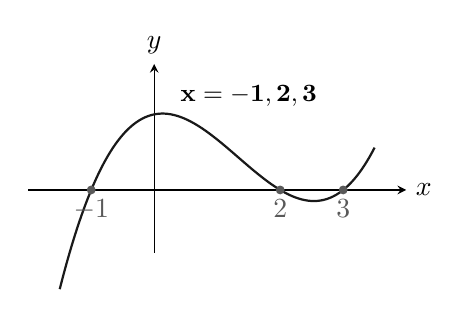
\begin{tikzpicture}[scale=0.8]
    \draw[->, >=stealth] (-2,0) -- (4,0) node[right] {$x$};
    \draw[->, >=stealth] (0,-1) -- (0,2) node[above] {$y$};
    \draw[thick, mainBlack, smooth, samples=100, domain=-1.5:3.5] plot (\x, {0.2*(\x+1)*(\x-2)*(\x-3)});
    
    \fill[subGray] (-1,0) circle (2pt) node[below] {$-1$};
    \fill[subGray] (2,0) circle (2pt) node[below] {$2$};
    \fill[subGray] (3,0) circle (2pt) node[below] {$3$};
    
    \node[align=center, font=\small] at (1.5, 1.5) {$\mathbf{x=-1, 2, 3}$};
\end{tikzpicture}
\end{center}

\talk{先生}{「計算上の『解』が、目の前で『座標』という実体を持ちましたね。これがデカルトの眼鏡を通した景色です」}

\newpage

% --- Page 2 ---
\subsection{Topic 2:重解と接点}

\talk{先生}{「では、この場合はどうでしょう?」}

先生は次の方程式とそのグラフを描いた。
\[ x^3 - 3x + 2 = 0 \]
\[ (x-1)^2(x+2) = 0 \]

\talk{私}{「因数分解すると $(x-1)^2$ が出てきます。つまり $x=1$ は重解ですね」}

\talk{先生}{「重解のとき、グラフはどうなっていますか?」}

\begin{center}
\begin{tikzpicture}[scale=0.8]
    \draw[->, >=stealth] (-3,0) -- (2,0) node[right] {$x$};
    \draw[->, >=stealth] (0,-1) -- (0,3) node[above] {$y$};
    \draw[thick, mainBlack, smooth, samples=100, domain=-2.5:1.5] plot (\x, {0.3*(\x-1)*(\x-1)*(\x+2)});
    
    \fill[subGray] (-2,0) circle (2pt) node[below left] {$-2$};
    \fill[subGray] (1,0) circle (2pt) node[below right] {$1$};
    
    \node[below, font=\small] at (-3.5, 1.0) {交わる (1重解)};
    \node[below, font=\small] at (1, -0.5) {\textbf{接する (重解)}};
\end{tikzpicture}
\end{center}

\talk{友人}{「あ、$x=1$ のところで山が地面にタッチしてる! 横切らずに跳ね返ってる感じ?」}

\talk{先生}{「その通り。解が重なるとき、グラフは $x$軸に\textbf{接し}ます。まるで2つの交点が1つに融合したかのように」}

\begin{SolidBox}
    \textbf{重解の幾何学的意味}
    \begin{itemize}
        \item 方程式が $(x-\alpha)^2$ を因数にもつ $\iff$ グラフは $x=\alpha$ で $x$軸に\textbf{接する}。
        \item 方程式が $(x-\alpha)^3$ を因数にもつ $\iff$ グラフは $x=\alpha$ で\textbf{接しながら突き抜ける}(3重解)。
    \end{itemize}
\end{SolidBox}



\subsection{Topic 3:見えない解の行方}

\talk{私}{「先生、じゃあ\textbf{虚数解}はどうなるんですか? 実数解が共有点なら、虚数解は?」}

\talk{先生}{「良い質問です。方程式 $x^3-1=0$ を例にとりましょう。解は実数の $1$ と、虚数の $\frac{-1\pm\sqrt{3}i}{2}$ でしたね」}

\talk{先生}{「グラフ $y=x^3-1$ を描いてごらんなさい」}

\begin{center}
\begin{tikzpicture}[scale=0.6]
    \draw[->, >=stealth] (-2,0) -- (2,0) node[right] {$x$};
    \draw[->, >=stealth] (0,-2) -- (0,2) node[above] {$y$};
    \draw[thick, mainBlack, smooth, samples=100, domain=-1.5:1.5] plot (\x, {\x*\x*\x - 1});
    \fill[subGray] (1,0) circle (2pt) node[below right] {$1$};
\end{tikzpicture}
\end{center}

\talk{友人}{「あれ? $x$軸と1回しかぶつかってない。$x=1$ だけだ」}

\talk{先生}{「そうです。我々が見ている実数のグラフ(xy平面)には、虚数解は映り込みません。虚数解とは、グラフが $x$軸と\textbf{出会えなかった}証拠なのです」}



\subsection{Epilogue:次元の狭間で}

グラフと方程式。二つの視点を行き来することで、数式の意味が立体的になってきた。

\talk{先生}{「共有点が見えれば解が見える。逆に、解の形(重解や虚数解)が分かれば、グラフの形状が見えてくる。この二つは表裏一体なのです」}

\talk{先生}{「さて、方程式という冒険もいよいよ大詰めです。次回は、この複素数の世界で最も美しく、不思議な数について語りましょう。1の3乗根、オメガの物語です」}

\vspace{2em}
\begin{center}
    \small \itshape To be continued in Lecture 9...
\end{center}

% =======================================================
% 第9回
% =======================================================
\newpage
\setcounter{section}{8} % 第9回
\setKey{The Cyclic Trinity}

\section{1の3乗根と複素数:循環する三位一体}

% --- Page 1 ---
\subsection{Prologue:1の正体}

「$1$ の $3$ 乗根を求めよ」
黒板にはシンプルな問いが書かれていた。

\talk{友人}{「え、そんなの $1$ に決まってるじゃん。$1 \times 1 \times 1 = 1$ でしょ? 秒殺!」}

友人は自信満々に答えるが、先生は静かに首を横に振った。

\talk{先生}{「実数の世界だけなら、その通りです。しかし、我々はもう『複素数』という広い海を知ってしまいました。方程式 $x^3 = 1$ は $3$ 次方程式です。ならば、解は必ず $3$ つあるはずですね?」}

\talk{私}{「あ……そうか。残り $2$ つは虚数の中に隠れているんですね」}

\talk{先生}{「その通り。今日は、その隠された兄弟たちを探しに行きましょう。彼らは驚くほど美しい性質を持っています」}

\subsection{Topic 1:オメガの誕生}

まず、方程式を変形して因数分解を行う。

\[ x^3 - 1 = 0 \iff (x-1)(x^2+x+1) = 0 \]

\talk{私}{「$x-1=0$ からは $x=1$ が出ます。残りは $x^2+x+1=0$ を解の公式で解けばいいんですね」}

\[ x = \frac{-1 \pm \sqrt{1^2 - 4}}{2} = \frac{-1 \pm \sqrt{3}i}{2} \]

\talk{先生}{「正解です。この虚数解のうちの一つを、ギリシャ文字の最後尾をとって $\mathbf{\omega}$(オメガ)と名付けましょう」}

\begin{SolidBox}
    \textbf{定義:1の3乗根 $\omega$}
    
    方程式 $x^3=1$ の虚数解の一つを $\omega$ とおく。
    \[ \omega = \frac{-1 + \sqrt{3}i}{2} \quad \left(\text{または } \frac{-1 - \sqrt{3}i}{2}\right) \]
\end{SolidBox}

% Ref: , 

\talk{友人}{「オメガ……なんか強そう。でもこれ、計算するの大変そうじゃない?」}

\talk{先生}{「いいえ、逆です。$\omega$ は『計算をサボるための記号』なのです。次の2つの性質を見てください」}

\subsection{Topic 2:最強の性質 2選}

先生は黒板に大きな円を描き、その円周上に $1, \omega, \omega^2$ を配置した。それは正三角形を成していた。

\begin{SolidBox}
    \textbf{$\omega$ の性質}
    \begin{enumerate}
        \item \textbf{3乗すると1に戻る}: $\mathbf{\omega^3 = 1}$
        \item \textbf{2乗と1乗と1を足すと0}: $\mathbf{\omega^2 + \omega + 1 = 0}$
    \end{enumerate}
\end{SolidBox}

% Ref: 

\talk{私}{「1番目は定義から当たり前ですが、2番目は? $\omega$ は $x^2+x+1=0$ の解だから……あ、代入すれば成り立ちますね!」}

\talk{先生}{「その通り。この2つの武器があれば、どんな高次式も瞬時に次数を下げられます」}

\begin{NoteBox}
    \textbf{例題:$\omega$ の計算}
    
    (1) $\omega^5$
    \[ \omega^5 = \omega^3 \cdot \omega^2 = 1 \cdot \omega^2 = \mathbf{\omega^2} \]
    
    (2) $\omega^4 + \omega^2 + 1$
    \[ \omega^4 = \omega^3 \cdot \omega = \omega \text{ なので、} \quad \omega + \omega^2 + 1 = \mathbf{0} \]
\end{NoteBox}

% Ref: , 

\talk{友人}{「うわ、本当だ! どんなに数字が大きくても、$3$ で割った余りだけ見ればいいんだ。循環してるってこと?」}

\talk{先生}{「そうです。$1 \to \omega \to \omega^2 \to 1 \dots$ と、永遠に回り続けるメリーゴーランドのような数。それが $\omega$ なのです」}

\newpage

% --- Page 2 ---
\subsection{Topic 3:複素数の範囲での因数分解}

\talk{先生}{「さて、視点を少し変えましょう。これまで『因数分解できない』と諦めていた式も、複素数を使えば無理やり分解できます」}

\begin{SolidBox}
    \textbf{複素数の範囲での因数分解}
    
    2次方程式 $ax^2+bx+c=0$ の解 $\alpha, \beta$ を求めれば、
    どんな式も $a(x-\alpha)(x-\beta)$ に分解できる。
\end{SolidBox}

% Ref: 

\talk{私}{「例えば、$x^2+4$ とかはどうなりますか?」}

\talk{先生}{「$x^2 = -4$ を解くと $x = \pm 2i$ ですね。したがって……」}

\[ x^2 + 4 = (x - 2i)(x + 2i) \]

\talk{私}{「なるほど。足し算の形でも、無理やり積の形にできるんですね」}

\subsection{Topic 4:3数を解とする方程式}

\talk{先生}{「最後に、解と係数の関係の『3次バージョン』を紹介しておきましょう。3つの数 $\alpha, \beta, \gamma$ を解に持つ方程式を作るには、どうすればいいでしょうか?」}

\talk{友人}{「$(x-\alpha)(x-\beta)(x-\gamma)=0$ を展開すればいいんじゃない?」}

\talk{先生}{「正解です。展開するとこうなります」}

\[ x^3 - (\alpha+\beta+\gamma)x^2 + (\alpha\beta+\beta\gamma+\gamma\alpha)x - \alpha\beta\gamma = 0 \]

% Ref: 

\talk{先生}{「和、2つずつの積の和、そして3つの積。このリズムは2次方程式の時と同じですね。係数は美しい対称性を持っているのです」}

\subsection{Epilogue:到達点へ}

黒板には $\omega$ の三角形と、因数分解された式たちが並んでいる。

\talk{先生}{「有理数、無理数、実数、そして虚数。我々は数を拡張するたびに、自由を手に入れてきました。解けない方程式はなくなり、因数分解できない式も消滅しました」}

先生はチョークを置き、私たちに向き直った。

\talk{先生}{「これで、『複素数と方程式』の単元における主な道具はすべて揃いました。次回は、これまでの知識を総動員して、自分の力がどこまで通用するかを試すときです」}

\talk{友人}{「え、まさかテスト?」}

\talk{先生}{「到達度確認テストです。恐れることはありません。君たちの手にはすでに、虚数という最強の武器があるのですから」}

\vspace{2em}
\begin{center}
    \small \itshape To be continued in Lecture 10...
\end{center}

% =======================================================
% 第10回
% =======================================================
\newpage
\setcounter{section}{9} % 第10回
\setKey{Crossing the Imaginary Line}

\section{到達度確認:虚数世界の歩き方}

% --- Page 1 ---
\subsection{Prologue:武器の点検}

教室の空気は少し張り詰めていた。机の上には、白いプリントが裏返しに置かれている。
「到達度確認テスト」。その文字が透けて見える。

\talk{先生}{「恐れることはありません。君たちはこの数週間で、数直線の外側に広がる広大な世界を旅してきました。その手には、もう十分な武器があるはずです」}

先生は黒板に、私たちが獲得してきた概念をキーワードとして書き並べた。
\begin{itemize}
    \item $i^2 = -1$ (虚数単位)
    \item $A=BQ+R$ (割り算の構造)
    \item 解と係数の関係 (対称性)
    \item 因数定理 $P(k)=0$ (次元の縮小)
    \item $\omega^3=1$ (循環)
\end{itemize}

\talk{先生}{「テストとは、敵を倒すためのものではなく、自分の武器が錆びついていないかを確認するための儀式です。さあ、始めましょう」}

\subsection{Trial 1:計算の迷宮}

\begin{NoteBox}
    \textbf{第1問 (複素数の計算)} \\
    次の計算をし、$a+bi$ の形で答えよ。
    \[ (1) \ (3-2i)^2 \quad\quad (2) \ \frac{5}{1-2i} \]
\end{NoteBox}

\talk{私}{(まずは基本計算だ。$(3-2i)^2$ は普通に展開して…… $i^2$ を $-1$ に変えるのを忘れずに)}
\begin{align*}
    (3-2i)^2 &= 9 - 12i + 4i^2 = 9 - 12i - 4 = \mathbf{5 - 12i}
\end{align*}

\talk{友人}{「割り算は『共役』を使うんだよね。分母が $1-2i$ だから、相棒の $1+2i$ を掛ければいい」}
\begin{align*}
    \frac{5(1+2i)}{(1-2i)(1+2i)} &= \frac{5(1+2i)}{1^2+2^2} = \frac{5(1+2i)}{5} = \mathbf{1+2i}
\end{align*}

\talk{先生}{「順調ですね。計算のルールは実数と同じ。ただ一つ、『$i^2$ は $-1$ になる』という魔法がかかっているだけです」}

\subsection{Trial 2:対称性の海}

\begin{NoteBox}
    \textbf{第2問 (解と係数の関係)} \\
    2次方程式 $x^2 - 3x + 4 = 0$ の2つの解を $\alpha, \beta$ とするとき、次の式の値を求めよ。
    \[ (1) \ \alpha^2 + \beta^2 \quad\quad (2) \ \frac{1}{\alpha} + \frac{1}{\beta} \]
\end{NoteBox}

\talk{私}{(解の公式を使って $\alpha, \beta$ を求めてから代入するのは……悪手だ。ここは『関係』を見る)}

私は反射的に和と積をメモした。
\[ \alpha+\beta = 3, \quad \alpha\beta = 4 \]

\talk{友人}{「あとはパズルだね。2乗の和は、和の2乗から邪魔な真ん中を引く!」}
\begin{itemize}
    \item $\alpha^2+\beta^2 = (\alpha+\beta)^2 - 2\alpha\beta = 3^2 - 2\cdot 4 = 9-8 = \mathbf{1}$
    \item $\frac{1}{\alpha} + \frac{1}{\beta} = \frac{\alpha+\beta}{\alpha\beta} = \mathbf{\frac{3}{4}}$
\end{itemize}

\talk{先生}{「素晴らしい。解そのものは汚い数字(虚数)かもしれませんが、それらが織りなす『対称式』の値は、こんなにも綺麗な整数になるのです」}

\newpage

% --- Page 2 ---
\subsection{Trial 3:方程式の復元}

\begin{NoteBox}
    \textbf{第3問 (因数定理と高次方程式)} \\
    3次方程式 $x^3 - 4x^2 + ax + b = 0$ が $x=1$ と $x=2$ を解にもつとき、定数 $a, b$ の値を求めよ。
\end{NoteBox}

\talk{友人}{「解ってことは、代入して成り立つってことだよね? 連立方程式にすれば解けそう」}

\begin{align*}
    x=1 \implies 1 - 4 + a + b = 0 &\iff a+b=3 \\
    x=2 \implies 8 - 16 + 2a + b = 0 &\iff 2a+b=8
\end{align*}
これを解いて $\mathbf{a=5, b=-2}$。

\talk{先生}{「正攻法ですね。では、もう少し視点を変えてみましょうか。解が $1$ と $2$ であるなら、この式は $(x-1)$ と $(x-2)$ を因数に持つはずです」}

\talk{私}{「あ、そうか! 展開して係数比較もできるんだ」}
\[ (x-1)(x-2)(x-\gamma) = x^3 - (\dots)\dots \]

\subsection{Trial 4:循環する魂}

\begin{NoteBox}
    \textbf{第4問 (高次方程式とオメガ)} \\
    (1) 4次方程式 $x^4 - 3x^2 - 4 = 0$ を解け。 \\
    (2) 方程式 $x^3=1$ の虚数解の一つを $\omega$ とするとき、$\omega^{5} + \omega^4 + 1$ の値を求めよ。
\end{NoteBox}

\talk{私}{((1)は複二次式だ。$x^2=X$ と置けば……)}
\[ X^2 - 3X - 4 = 0 \implies (X-4)(X+1) = 0 \]
$X = 4, -1$ だから、$x^2=4$ と $x^2=-1$。
実数解 $\pm 2$ と、虚数解 $\pm i$。答えは $\mathbf{x = \pm 2, \pm i}$。

\talk{友人}{((2)はオメガ! 3回掛けたら1に戻るやつ!)}
\[ \omega^5 = \omega^3 \cdot \omega^2 = \omega^2 \]
\[ \omega^4 = \omega^3 \cdot \omega = \omega \]
よって与式は $\omega^2 + \omega + 1$。これはオメガの性質そのものだから…… $\mathbf{0}$!

\subsection{Epilogue:実数への帰還}

チャイムが鳴り、答案用紙が回収されていく。
難解に見えた記号の羅列が、今では意味を持った「言葉」として読めるようになっていた。

\talk{先生}{「お疲れ様でした。これで、我々の『複素数と方程式』の旅は一区切りです。君たちは数直線を飛び出し、虚数の海を渡り、方程式という島を制圧しました」}

先生は教卓でプリントを整えながら、ふと真面目な顔つきになった。

\talk{先生}{「しかし、この広大な複素数の世界には、一つだけ欠けているものがあります」}

\talk{友人}{「欠けているもの?」}

\talk{先生}{「そうです。君たちは $\omega$ と $i$ のどちらが大きいか、答えられますか?」}

私たちは顔を見合わせた。答えられない。複素数には大小関係がないからだ。

\talk{先生}{「完全無欠に見える複素数も、『順序』という秩序を持たないのです。次回からは、我々が元いた場所——\textbf{実数(Real Number)}の世界に戻ります」}

\talk{私}{「実数に戻って、何をするんですか?」}

\talk{先生}{「大小関係があるからこそできること。すなわち『証明』です。『どちらが大きいか』を論理的に語る技術。それは虚数の世界では得られなかった、実数だけの特権なのです」}

窓の外、現実の夕日が校庭を赤く染めている。
魔法のような虚数の時間は終わり、厳格な論理の時間が始まろうとしていた。

\vspace{2em}
\begin{center}
    \small \itshape To be continued in Lecture 11 (Part II: Proofs and Logic)...
\end{center}

% =======================================================
% 第11回
% =======================================================
\newpage
\setcounter{section}{10} % 第11回
\setKey{The Art of Logic}

\section{等式の証明:論理という名の言語}

% --- Page 1 ---
\subsection{Prologue:当たり前を疑う}

「証明しなさい」
数学のプリントにその言葉が現れると、私はいつも少し身構えてしまう。
$(a+b)^2 = a^2+2ab+b^2$ を証明せよ、と言われても、「展開したらそうなるじゃん」以外の言葉が見つからないのだ。

\talk{私}{「先生、明らかに正しい式をわざわざ証明する意味って何ですか? 見れば分かると思うんですが」}

\talk{先生}{「『見れば分かる』は危険な言葉です。君が見ているのは、たまたま上手くいった数例かもしれません。証明とは、\textbf{誰が、いつ、どこで計算しても絶対にそうなる}ことを、論理の鎖で保証する手続きなのです」}

先生は黒板に $A=B$ と大きく書いた。

\talk{先生}{「今日から我々は『式と証明』の章に入ります。計算して答えを出す『探検』から、そのルートが正しいことを説明する『地図作り』へと、頭の使い方をシフトしてください」}

\subsection{Topic 1:証明の作法}

\talk{先生}{「まず、絶対にやってはいけない禁じ手から教えましょう。証明したい式を、最初から『=』で結んで書いてはいけません」}

\talk{友人}{「えっ、ダメなの? $A=B$ を証明しろって言われたら、1行目に $A=B$ って書きたくなるけど」}

\talk{先生}{「それは『結論』です。まだ正しいと分かっていない式を、さも正しいかのように使ってはいけません。等式の証明には、主に3つの正規ルートがあります」}

\newpage

\begin{SolidBox}
    \textbf{等式 $A=B$ を証明する3つのアプローチ}
    \begin{enumerate}
        \item \textbf{一方変形型}:複雑な方の辺を変形して、シンプルな方の辺に変える。
        \[ \text{左辺} = \cdots = \cdots = \text{右辺} \]
        \item \textbf{両辺変形型}:左辺と右辺をそれぞれ変形し、同じ着地点(式)にたどり着く。
        \[ \text{左辺} = \cdots = C, \quad \text{右辺} = \cdots = C \]
        \item \textbf{引き算型}:$A-B$ を計算し、すべてが消えて $0$ になることを示す。
        \[ \text{左辺} - \text{右辺} = \cdots = 0 \]
    \end{enumerate}
\end{SolidBox}

\talk{私}{「なるほど……。ゴールテープは最後に切らないといけないんですね」}

\talk{先生}{「その通り。では、例題で練習してみましょう」}

\begin{NoteBox}
    \textbf{例題} \\
    等式 $a^3+b^3=(a+b)^3-3ab(a+b)$ を証明せよ。
\end{NoteBox}

\talk{友人}{「右辺の方がごちゃごちゃしてるから、右辺を計算して左辺にすればいいかな」}

\begin{align*}
    (\text{右辺}) &= (a^3 + 3a^2b + 3ab^2 + b^3) - (3a^2b + 3ab^2) \\
    &= a^3 + b^3 \\
    &= (\text{左辺}) \quad \text{// 証明終了}
\end{align*}

\talk{先生}{「完璧です。これが最も基本的で美しい証明の形です」}

\newpage

\subsection{Topic 2:条件付きの等式}

\talk{先生}{「次は、条件がついている場合です。例えば、『$a+b+c=0$ のとき』という条件があったら、どう使いますか?」}

\talk{私}{「$c = -a-b$ と変形して、式の中の $c$ を全部消したくなります」}

\talk{先生}{「良い直感です。条件式は\textbf{文字を減らすための道具}です。変数を減らせば、式は扱いやすくなります」}

\begin{NoteBox}
    \textbf{例題} \\
    $a+b+c=0$ のとき、等式 $a^3+b^3+c^3=3abc$ を証明せよ。
\end{NoteBox}

\talk{友人}{「うわ、有名な式だ。でもこれ、$c$ に $(-a-b)$ を代入して計算するの? めちゃくちゃ大変そう……」}

\talk{先生}{「計算力も数学の筋肉の一つですよ。しかし、因数分解の公式を知っていれば、一瞬で終わる話でもあります」}

\begin{align*}
    a^3+b^3+c^3 - 3abc &= (a+b+c)(a^2+b^2+c^2-ab-bc-ca) \\
    &= 0 \cdot (\dots) \\
    &= 0
\end{align*}

\talk{先生}{「条件 $a+b+c=0$ があるので、右辺は丸ごと消滅します。よって $a^3+b^3+c^3 - 3abc = 0$、すなわち証明完了です」}



\subsection{Topic 3:比例式の定石}

最後に先生は、分数の形をした等式(比例式)を板書した。

\[ \frac{a}{b} = \frac{c}{d} \]

\talk{先生}{「この形を見たら、条件反射でやるべきことがあります。それは、\textbf{『=k』と置く}ことです」}

\begin{SolidBox}
    \textbf{比例式の扱い方}
    
    \[ \frac{a}{b} = \frac{c}{d} = k \quad \Longrightarrow \quad a=bk, \ c=dk \]
    
    文字を $b, d, k$ の3種類に統一できる。
\end{SolidBox}



\talk{私}{「$a$ と $c$ を消去して、$k$ の式にしちゃうんですね」}

\talk{先生}{「そうです。左辺も右辺も計算すると結局 $k$ になる、という『両辺変形型』で証明するのが定石です。文字が増えたように見えて、実は変数の自由度は下がっているのがポイントです」}

\subsection{Epilogue:厳密さの先へ}

ノートには「左辺=……=右辺」という整然とした式変形が並んだ。
計算の羅列に見えるが、そこには「迷いなくゴールへ進む」という強い意志が込められている。

\talk{先生}{「等式の証明は、論理の基礎トレーニングです。しかし、世界は『等しい』関係ばかりではありません。むしろ『どちらかが大きい』という不平等な関係の方が多い」}

先生は窓の外を指差した。

\talk{先生}{「次回は、いよいよ実数の本質である\textbf{『大小関係』}に踏み込みます。不等式の証明。そこでは、『=0』ではなく『>0』を示すための、新しい技術が必要になります」}

\talk{友人}{「不等式かぁ……。等式より難しそうだね」}

\talk{私}{「でも、実数の世界に帰ってきた感じがするよ」}

私たちは、大小のある世界へと足を踏み入れる準備を整えた。

\vspace{2em}
\begin{center}
    \small \itshape To be continued in Lecture 12...
\end{center}

% =======================================================
% 第12回
% =======================================================
\newpage
\setcounter{section}{11} % 第12回
\setKey{The Privilege of Reality}

\section{不等式の証明(1):実数だけの特権}

% --- Page 1 ---
\subsection{Prologue:順序のある世界}

「どちらが大きいか?」
この問いは、単純に見えて奥が深い。
先生は黒板に $i$ と $2i$ を書き、私たちに問いかけた。

\talk{先生}{「前回、虚数には大小関係がないと言いましたね。もし $i > 0$ だとしたら、両辺に $i$ を掛けると $-1 > 0$ という矛盾が生まれてしまうからです」}

\talk{私}{「つまり、不等号 $>, <$ が使えるのは、実数の世界だけなんですね」}

\talk{先生}{「その通り。不等式とは、数が直線上に一列に並んでいる実数世界だけの特権的な言語なのです。今日はその『順序』を、論理的に証明する方法を学びます」}

\subsection{Topic 1:比較の基準}

先生は黒板に $A > B$ と書き、チョークを置いた。

\talk{先生}{「$A$ が $B$ より大きいことを証明しなさい、と言われたら、君たちはどうしますか? グラフを描きますか? 具体的な数値を入れますか?」}

\talk{友人}{「うーん、グラフは面倒だし……単純に引き算すればいいんじゃない? $A$ から $B$ を引いて、プラスになれば勝ち、みたいな」}

\talk{先生}{「正解です。二つの異なる数を比較するのは大変ですが、『ある数が $0$ より大きいかどうか』を調べるのは簡単です。基準を $0$ に持ってくるのです」}

\begin{SolidBox}
    \textbf{不等式証明の基本原理}
    
    \[ A > B \iff \boldsymbol{A - B > 0} \]
    
    証明の第一歩は、迷わず\textbf{「左辺 $-$ 右辺」}を計算することである。
\end{SolidBox}



\subsection{Topic 2:積の形を作る}

\talk{先生}{「では、具体的な問題を解いてみましょう。引き算をした後、どうすれば『正である』と言えるのか。そこが腕の見せ所です」}

\begin{NoteBox}
    \textbf{例題 1} \\
    $a>b$ かつ $x>y$ のとき、次の不等式を証明せよ。
    \[ ax + by > ay + bx \]
\end{NoteBox}

\talk{私}{「とりあえず、引いてみます。$(\text{左辺}) - (\text{右辺}) = ax + by - ay - bx$」}

私はノートの上で項を並べ替える。$a$ でくくって、$b$ でくくって……。

\begin{align*}
    ax + by - ay - bx &= a(x-y) - b(x-y) \\
    &= (a-b)(x-y)
\end{align*}

\talk{友人}{「あ、因数分解できた! これなら符号が分かるよ」}

\talk{先生}{「その通り。条件 $a>b, x>y$ より、$a-b>0$ かつ $x-y>0$ ですね。プラス $\times$ プラスは?」}

\talk{私}{「プラス、つまり $>0$ です」}

\talk{先生}{「よって $(\text{左辺}) - (\text{右辺}) > 0$ が示せました。これで証明完了です。バラバラの項のままでは符号が分からなくても、\textbf{因数分解して積の形にすれば}符号が判定できる。これが定石です」}



\subsection{Topic 3:条件というヒント}

\talk{先生}{「次は、条件式が少し変わった形をしている場合です。『$1$ より大きい』という条件をどう使うか」}

\begin{NoteBox}
    \textbf{例題 2} \\
    $a>1, \ b>1$ のとき、不等式 $ab + 1 > a + b$ を証明せよ。
\end{NoteBox}

\talk{友人}{「$a>1$ ってことは、$a$ に $2$ とか $3$ を入れれば成り立つのは分かるけど……証明となるとどう書けばいいの?」}

\talk{先生}{「不等式の証明において、条件式は『変形して符号を作る』ためにあります。$a>1$ ならば $a-1>0$ ですね。計算結果に $(a-1)$ が現れることを期待して、引き算してみましょう」}

私は祈るような気持ちで計算を始めた。

\begin{align*}
    (\text{左辺}) - (\text{右辺}) &= ab + 1 - a - b \\
    &= a(b-1) - (b-1) \quad (\leftarrow \text{$1-b$ をマイナスでくくる}) \\
    &= (a-1)(b-1)
\end{align*}

\talk{私}{「出ました! $(a-1)$ と $(b-1)$!」}

\talk{先生}{「素晴らしい。条件より $a-1>0, b-1>0$ ですから、その積も正になります。パズルのピースがカチッとはまるような快感でしょう?」}



\subsection{Epilogue:因数分解の限界}

黒板には、「引いて因数分解する」という美しい流れが記されている。
しかし、先生は少し意地悪な笑みを浮かべた。

\talk{先生}{「今回は、上手く因数分解できるケースばかりを扱いました。しかし、世の中には因数分解できない式の方が多いのです」}

先生は黒板の隅に $x^2 - 4x + 5$ と書いた。

\talk{先生}{「これ、因数分解できませんよね。でも、常に正の値をとります。なぜだか分かりますか?」}

\talk{私}{「ええと……平方完成すると $(x-2)^2 + 1$ だから、ですか?」}

\talk{先生}{「その通り! 実数のもう一つの強力な性質、『\textbf{2乗すると必ず0以上になる}』。次回はこの性質を使って、より手強い不等式を証明していきましょう」}

\vspace{2em}
\begin{center}
    \small \itshape To be continued in Lecture 13...
\end{center}

% =======================================================
% 第13回
% =======================================================
\newpage
\setcounter{section}{12} % 第13回
\setKey{The Power of Squares}

\section{不等式の証明(2):完全なる平方}

% --- Page 1 ---
\subsection{Prologue:実数最強の盾}

「絶対に負けない」
そんな言葉を数学的に表現するとしたら、どうなるだろうか。

\talk{先生}{「前回、因数分解によって符号を調べる方法を学びました。しかし、世の中には因数分解できない式の方が多いのです」}

先生は黒板に $x^2 - 4x + 6$ と書いた。

\talk{私}{「因数分解できませんね。解の公式を使うと虚数解になってしまいます」}

\talk{先生}{「虚数解になるということは、グラフが $x$ 軸と交わらない、つまり常に浮いているということです。この式が『常にプラスである』ことを、グラフを使わずに論理だけで示せますか?」}

\talk{友人}{「数値を代入してみる? $1$ でも $0$ でもプラスだけど……全部の数を試すわけにはいかないし」}

\talk{先生}{「そこで登場するのが、実数が持つ最強の盾です。どんな数も、2回掛ければ正義になる」}

\subsection{Topic 1:平方完成という技術}

\begin{SolidBox}
    \textbf{実数の基本性質}
    
    実数 $A$ について、常に次が成り立つ。
    \[ \boldsymbol{A^2 \geqq 0} \]
    (等号成立は $A=0$ のときのみ)
\end{SolidBox}



\talk{先生}{「マイナス $\times$ マイナスはプラス。この単純なルールが、証明においては絶大な力を発揮します。先ほどの式を変形してみましょう」}

\begin{align*}
    x^2 - 4x + 6 &= (x^2 - 4x + 4) + 2 \\
    &= (x-2)^2 + 2
\end{align*}

\talk{私}{「平方完成ですね。$(x-2)^2$ は絶対に $0$ 以上だから……それに $2$ を足せば、確実にプラスだ!」}

\begin{NoteBox}
    $(x-2)^2 \geqq 0$ なので、$(x-2)^2 + 2 \geqq 2 > 0$。
    よって、$x^2 - 4x + 6 > 0$ は常に成り立つ。
\end{NoteBox}



\talk{先生}{「その通り。正体不明だった式を『2乗の形』に押し込めることで、その非負性を暴き出す。これが平方完成の真の目的です」}

\subsection{Topic 2:2変数のダンス}

\talk{先生}{「では、変数を増やしてみましょう。$x^2 + y^2$ と $2xy$。どちらが大きいと思いますか?」}

\talk{友人}{「えー、数によるんじゃない? $x=1, y=2$ なら $1+4=5$ と $2\cdot1\cdot2=4$ で、左の方が大きいけど」}

\talk{先生}{「直感を信じて証明してみましょう。不等式の基本通り、引き算を行います」}

\[ (\text{左辺}) - (\text{右辺}) = x^2 + y^2 - 2xy \]

\talk{私}{「あ! これ、因数分解の公式そのままだ」}

\[ = (x-y)^2 \]

\talk{先生}{「美しいでしょう? ここでもやはり『2乗』が現れました。$x, y$ がどんな実数であっても、その差の2乗は決してマイナスになりません」}

\begin{SolidBox}
    \textbf{不等式の証明}
    
    \[ x^2 + y^2 \geqq 2xy \]
    
    証明:
    $(x^2 + y^2) - 2xy = (x-y)^2 \geqq 0$
    よって $x^2 + y^2 \geqq 2xy$。
\end{SolidBox}



\talk{私}{「もしこれ、$x$ や $y$ が虚数だったらどうなりますか?」}

\talk{先生}{「鋭い質問です。例えば $x=i, y=0$ とすると、左辺は $-1$、右辺は $0$ となり、不等式は成り立ちません。実数条件があるからこそ、我々はこの不等式を信じることができるのです」}



\subsection{Topic 3:等号が成立する瞬間}

\talk{先生}{「さて、不等式にはもう一つ、大事な視点があります。『いつ等しくなるのか』です」}

\talk{友人}{「等号成立条件ってやつですね。この問題なら $(x-y)^2 = 0$ になるときだから……」}

\talk{私}{「中身が $0$、つまり $x-y=0$ のときですね」}

\talk{先生}{「正解です。$x=y$ のとき、そしてそのときだけ、左辺と右辺は完全にバランスします。最大・最小問題を考えるとき、この『等号成立』の瞬間こそが、最も重要なポイントになります」}



\subsection{Epilogue:次なる高みへ}

黒板には、$( \quad )^2 \geqq 0$ を利用した証明が並んでいる。
単純な引き算から始まり、因数分解、そして平方完成へ。
私たちは「正であることを示す」ための道具を一つずつ増やしている。

\talk{先生}{「2乗して足す。これはとても強力な手法ですが、式が複雑になると計算が大変になりますね。実は、もっとエレガントに、魔法のように大小関係を見抜く『平均』の定理が存在します」}

\talk{友人}{「魔法?」}

\talk{先生}{「ええ。足して2で割る平均と、掛けてルートを取る平均。この二つの間には、決して覆らない絶対的な上下関係があるのです」}

先生はチョークを置き、楽しげに予告した。

\talk{先生}{「次回、不等式の王様、『相加・相乗平均の関係』についてお話ししましょう」}

\vspace{2em}
\begin{center}
    \small \itshape To be continued in Lecture 14...
\end{center}

% =======================================================
% 第14回
% =======================================================
\newpage
\setcounter{section}{13} % 第14回
\setKey{The Harmony of Means}

\section{相加・相乗平均:二つの中心}

% --- Page 1 ---
\subsection{Prologue:平均の顔つき}

「平均点を計算する」
そう言われたら、誰でも全部足して個数で割るだろう。

\talk{友人}{「$a$ と $b$ の平均は $\frac{a+b}{2}$。これ以外に平均なんてあるの?」}

\talk{先生}{「ありますよ。君たちが普段使っているのは\textbf{相加平均(Arithmetic Mean)}。しかし、世界には掛け算の世界の平均、\textbf{相乗平均(Geometric Mean)}も存在します」}

先生は黒板に $\sqrt{ab}$ と書いた。

\talk{私}{「足して $2$ で割るのが真ん中なら、掛けてルートを取るのも、ある意味『真ん中』なんですか?」}

\talk{先生}{「ええ。例えば $1$ と $100$ の真ん中は? 足せば $50.5$ ですが、倍率で見れば $1$ の $10$ 倍が $10$、$10$ の $10$ 倍が $100$。感覚的には $10$ も真ん中でしょう?」}

\talk{先生}{「そしてこの二つの平均の間には、決して覆らない厳格な上下関係が存在するのです」}

\subsection{Topic 1:絶対的な不等式}

先生は半円の図を描き始めた。

\begin{center}
\begin{tikzpicture}[scale=1.5]
    % Coordinates
    \coordinate (O) at (0,0);
    \coordinate (L) at (-2,0);
    \coordinate (R) at (2,0);
    \coordinate (M) at (0.5,0); % Split point
    
    % Semicircle
    \draw[thick, mainBlack] (R) arc (0:180:2);
    \draw[thick, mainBlack] (L) -- (R);
    
    % Radius (Arithmetic Mean)
    \draw[->, thick, subGray] (O) -- (0,2) node[midway, left] {半径 $\frac{a+b}{2}$};
    
    % Perpendicular (Geometric Mean)
    \draw[dashed] (M) -- (M |- 0,1.936);
    \draw[->, thick, mainBlack] (M) -- (0.5, {sqrt(1.5*2.5)}) node[midway, right] {垂線 $\sqrt{ab}$};
    
    % Labels
    \node[below] at (-0.75, 0) {$a$};
    \node[below] at (1.25, 0) {$b$};
    \node[below] at (O) {中心};
    \fill (O) circle (1pt);
\end{tikzpicture}
\end{center}

\talk{先生}{「直径を $a+b$ とすると、半径は $\frac{a+b}{2}$ です。一方、弦から立ち上がる垂線の長さは $\sqrt{ab}$ になります。図を見てごらんなさい。どちらが長いですか?」}

\talk{友人}{「半径の方が長い! ……あ、でも真ん中で重なるときだけ同じ長さになる?」}

\talk{先生}{「その通り。それが\textbf{等号成立}の瞬間です」}

\begin{SolidBox}
    \textbf{定理:相加平均と相乗平均の大小関係}
    
    $a > 0, \ b > 0$ のとき、
    \[ \frac{a+b}{2} \geqq \sqrt{ab} \quad \iff \quad \boldsymbol{a+b \geqq 2\sqrt{ab}} \]
    等号が成立するのは $\boldsymbol{a=b}$ のときである。
\end{SolidBox}


\talk{私}{「$a, b$ がプラスじゃないとダメなんですか?」}

\talk{先生}{「ルートの中がマイナスになっては困りますし、長さの話ですからね。この不等式を使うときは、必ず\textbf{『正の数である』}ことの確認が必要です」}

% =======================================================
% 第14回 (修正版)
% =======================================================

\subsection{Topic 2:最小値の罠}

\talk{先生}{「さて、この不等式が真価を発揮するのは、変数が消えて定数になるときです。例えば、$x$ とその逆数 $\frac{1}{x}$ の和を考えてみましょう」}

\begin{NoteBox}
    \textbf{例題 1} \\
    $x > 0$ のとき、$x + \frac{4}{x}$ の最小値を求めよ。
\end{NoteBox}

\talk{私}{「相加・相乗平均の関係を使えば、$x$ が消えそうです」}

\begin{align*}
    x + \frac{4}{x} &\geqq 2\sqrt{x \cdot \frac{4}{x}} \\
    &= 2\sqrt{4} \\
    &= 4
\end{align*}

\talk{友人}{「計算できた! 『4以上』ってことだから、最小値は 4 でしょ?」}

\talk{先生}{「待ちなさい。そこで思考停止してはいけません。\textbf{『4以上である』ことと、『最小値が4である』ことはイコールではない}のです」}

先生は教室を見渡し、例え話を始めた。

\talk{先生}{「例えば、『このクラスの生徒は全員 15歳以上である』というデータがあったとしましょう。では、このクラスの\textbf{最年少}は 15歳ですか?」}

\talk{友人}{「え? ……あ、そうとは限らないか。全員が 16歳以上かもしれないし。たまたま 15歳の人がいなければ、最年少は 15歳じゃない」}

\talk{先生}{「その通りです。最年少が 15歳だと断言するためには、実際に\textbf{『私が15歳です』と手を挙げる生徒}が存在しなければなりません」}

\talk{私}{「つまり、計算で『4以上』が出ても、実際に『値が4になる瞬間』があるか確かめないと、最小値とは言えないんですね」}

\talk{先生}{「そうです。この確認作業こそが\textbf{等号成立条件のチェック}です。実際に手を挙げる $x$ を探しましょう」}

\[ x = \frac{4}{x} \iff x^2 = 4 \]

$x>0$ より $x=2$。
実数 $x=2$ が確かに存在する。ここで初めて、「最小値は 4」と確定印が押されるのだ。

\begin{SolidBox}
    \textbf{最小値問題の鉄則}
    
    不等式 $A \geqq m$ を導いただけでは、最小値が $m$ とは限らない。
    \textbf{等号 $A=m$ を満たす実数が存在して}初めて、最小値 $m$ が確定する。
\end{SolidBox}


\subsection{Topic 3:存在の証明}

\talk{先生}{「この『存在確認』の意識を持って、次の問題を見てみましょう」}

\[ x > -2 \text{ のとき、 } x + \frac{9}{x+2} \text{ の最小値を求めよ。} \]

\talk{私}{「まずは形を揃えて、定数を作ります」}

\begin{align*}
    x + \frac{9}{x+2} &= (x+2) + \frac{9}{x+2} - 2 \\
    &\geqq 2\sqrt{(x+2) \cdot \frac{9}{x+2}} - 2 \\
    &= 2\sqrt{9} - 2 \\
    &= 4
\end{align*}

\talk{私}{「計算上は『4以上』になりました。でも、まだ答えじゃない。実際に 4 になれるか確認します」}

等号成立は、足した2つのパーツが等しいときだ。

\[ x+2 = \frac{9}{x+2} \]

これを解くと $(x+2)^2 = 9$。
$x>-2$ より $x+2 > 0$ なので、$x+2 = 3$。つまり $\mathbf{x=1}$。

\talk{友人}{「$x=1$ は条件 ($x>-2$) を満たしてる! ちゃんと存在するね」}

\talk{先生}{「よろしい。実数 $x=1$ という『証人』が見つかりました。よって自信を持って、最小値は 4 と答えてよいのです」}

\newpage


\subsection{Epilogue:最大と最小の狭間で}

黒板には、等号成立条件を確認する式が、単なるオマケではなく「証明の要」として強調されている。

\talk{先生}{「相加・相乗平均の関係は強力ですが、それゆえに『等号が成り立たない(値が存在しない)』という落とし穴も多い。常に『その値になる実数はあるか?』と問いかける癖をつけてください」}

\talk{先生}{「さて、変数が2つの場合の絶対不等式を見てきましたが、世の中には、ベクトルと深く関わるもう一つの強力な不等式が存在します」}

\talk{私}{「ベクトル……?」}

\talk{先生}{「次回は、不等式界のもう一人の巨人、『コーシー・シュワルツの不等式』を紹介しましょう」}

\vspace{2em}
\begin{center}
    \small \itshape To be continued in Lecture 15...
\end{center}


% =======================================================
% 第15回
% =======================================================
\newpage
\setcounter{section}{14} % 第15回
\setKey{Vectors in Disguise}
\section{発展:コーシー・シュワルツの不等式}

% --- Page 1 ---
\subsection{Prologue:最強の盾、再臨}

黒板には、相加・相乗平均の半円の図がまだ薄く残っている。
先生はそれを消し、代わりに少し長めの式を書き始めた。

\[ (a^2+b^2)(x^2+y^2) \geqq (ax+by)^2 \]

\talk{私}{「うわ、なんか強そうな式ですね。2乗がいっぱい……」}

\talk{友人}{「左側は、それぞれの2乗を足してから掛ける。右側は、混ぜてから2乗する。計算したら右の方が大きくなりそうじゃない?」}

\talk{先生}{「直感は大切ですが、この式に関しては逆です。『混ぜる前に強めた方が強い』のです。この不等式は、数学の世界で最も美しく、最も頻繁に使われる定理の一つ。\textbf{コーシー・シュワルツの不等式}といいます」}

\subsection{Topic 1:構造の証明}

\begin{SolidBox}
    \textbf{定理:コーシー・シュワルツの不等式}
    
    実数 $a, b, x, y$ について、常に次が成り立つ。
    \[ \boldsymbol{(a^2+b^2)(x^2+y^2) \geqq (ax+by)^2} \]
    等号が成立するのは $\boldsymbol{ay=bx}$ のときである。
\end{SolidBox}

% Ref: 

\talk{先生}{「証明の方法は一つ。我々の定石通り、『引いて符号を調べる』です」}

\talk{私}{「左辺から右辺を引くんですね。展開が大変そうですけど……やってみます」}

私はノートに計算を展開していく。

\begin{align*}
    (\text{左辺}) - (\text{右辺}) &= (a^2x^2 + a^2y^2 + b^2x^2 + b^2y^2) - (a^2x^2 + 2abxy + b^2y^2) \\
    &= a^2y^2 - 2abxy + b^2x^2
\end{align*}

\talk{友人}{「あれ? $a^2x^2$ と $b^2y^2$ が消えて……残ったこれ、因数分解できる!」}

\[ = (ay - bx)^2 \]

\talk{私}{「おおっ! 2乗の形になりました。実数の2乗だから、絶対に $0$ 以上です!」}

\talk{先生}{「その通り。複雑に見える式も、差を取れば一つの完全平方式に収束する。この数式の精巧なパズルこそが、コーシー・シュワルツの美しさです」}

% Ref: , 

\subsection{Topic 2:ベクトルの影}

先生は黒板の隅に、2本の矢印を描いた。

\talk{先生}{「実はこの不等式、君たちが将来学ぶ(あるいは物理で見たことがあるかもしれない)『ベクトル』の言葉で翻訳すると、当たり前のことを言っているに過ぎません」}

\begin{NoteBox}
    ベクトル $\vec{u} = (a, b)$、$\vec{v} = (x, y)$ とすると、
    \begin{itemize}
        \item 大きさの2乗: $|\vec{u}|^2 = a^2+b^2, \quad |\vec{v}|^2 = x^2+y^2$
        \item 内積: $\vec{u} \cdot \vec{v} = ax+by$
    \end{itemize}
    不等式は $\boldsymbol{|\vec{u}|^2 |\vec{v}|^2 \geqq (\vec{u} \cdot \vec{v})^2}$ を意味する。
\end{NoteBox}

% Ref: 

\talk{先生}{「内積の公式 $\vec{u} \cdot \vec{v} = |\vec{u}| |\vec{v}| \cos\theta$ を思い出せば、これは $(\cos\theta)^2 \leqq 1$ という、極めて当然の事実なのです」}

\talk{友人}{「へえー! 図形的な意味があるんだ。だから『シュワルツ』なんて強そうな名前がついてるのね」}

\subsection{Topic 3:最大値と最小値の同時捕獲}

\talk{先生}{「さて、この不等式の凄いところは、条件付きの最大・最小問題を一撃で仕留められる点です」}

\begin{NoteBox}
    \textbf{例題} \\
    $x^2 + y^2 = 4$ のとき、$3x + 4y$ の最大値と最小値を求めよ。
\end{NoteBox}

\talk{私}{「$y$ を消去して2次方程式の判別式で解く……とかですか?」}

\talk{先生}{「それも正攻法ですが、計算が少し重いですね。コーシー・シュワルツの不等式の『形』に合わせてごらんなさい。$a=3, b=4$ と見なすのです」}

\begin{align*}
    (3^2+4^2)(x^2+y^2) &\geqq (3x+4y)^2 \\
    25 \cdot 4 &\geqq (3x+4y)^2 \\
    100 &\geqq (3x+4y)^2
\end{align*}

\talk{友人}{「えっ、これで終わり? 2乗して $100$ 以下ってことは……」}

\[ -10 \leqq 3x+4y \leqq 10 \]

\talk{先生}{「はい、終了です。最大値 $10$、最小値 $-10$。幾何学的には、円と直線の接する位置を計算していることになります」}

% Ref: , 

\subsection{Epilogue:拡張する世界}

\talk{先生}{「この不等式は、変数が3つになっても、4つになっても、あるいは $n$ 個になっても成り立ちます」}

\[ (a^2+b^2+c^2)(x^2+y^2+z^2) \geqq (ax+by+cz)^2 \]

\talk{先生}{「次元が増えても壊れない強固な構造。それが実数の世界の秩序です」}

先生は満足げに黒板を眺めた。

\talk{先生}{「さて、長かった『式と証明』の旅も、いよいよフィナーレが近づいてきました。次回は、これまでの全ての知識——等式、不等式、複素数、因数分解——を総動員して、単元の総整理を行います」}

\talk{私}{「いよいよ、ラスボス戦ですね」}

\talk{先生}{「ええ。ですが今の君たちなら、どんな問題も論理の力でねじ伏せることができるはずです」}

\vspace{2em}
\begin{center}
    \small \itshape To be continued in Lecture 16...
\end{center}

% =======================================================
% 第16回
% =======================================================
\newpage
\setcounter{section}{15} % 第16回
\setKey{The Map of Numbers}

\section{単元の総整理(1):地図を描く}

% --- Page 1 ---
\subsection{Prologue:旅の軌跡}

黒板には、一枚の大きな地図が描かれていた。
左側には「実数の大陸」、右側には「複素数の海」。そしてその間には、方程式や不等式という橋が架かっている。

\talk{先生}{「我々は長い旅をしてきました。式の計算から始まり、虚数の海へ漕ぎ出し、方程式という島々を巡り、そして実数の大陸へ戻って論理の城(証明)を築きました」}

\talk{私}{「こうして見ると、全然違うことをやっていたようで、全部繋がっているんですね」}

\talk{先生}{「その通りです。今日は、この旅で得た知識を整理し、頭の中に『数学の地図』を完成させましょう。個別のテクニックではなく、構造を理解するのです」}

\subsection{Topic 1:二つの世界の掟}

先生は黒板の中央に線を引いた。

\talk{先生}{「まず、我々が行き来した二つの世界の違いを明確にしましょう。実数 $\mathbb{R}$ と複素数 $\mathbb{C}$。それぞれの世界の『掟』は何でしたか?」}

\talk{友人}{「実数の世界は……『2乗したらプラス』で、『大小関係がある』!」}

\talk{先生}{「正解です。では複素数の世界は?」}

\talk{私}{「2乗してマイナスになる数があって、大小関係がない。でも、方程式は必ず解ける」}

\newpage

\begin{SolidBox}
    \textbf{世界の比較:Real vs Complex}
    \begin{center}
    \begin{tabular}{c|c|c}
         & \textbf{実数の世界 ($\mathbb{R}$)} & \textbf{複素数の世界 ($\mathbb{C}$)} \\ \hline
        \textbf{2乗すると} & 必ず $x^2 \geqq 0$ & 負になることもある ($i^2=-1$) \\ \hline
        \textbf{大小関係} & ある ($>$, $<$, $\geqq$) & \textbf{ない} (定義できない) \\ \hline
        \textbf{方程式の解} & 解なしの場合あり & $n$次方程式は必ず$n$個持つ \\ \hline
        \textbf{主な活動} & 不等式の証明 & 等式の証明・値の計算 \\
    \end{tabular}
    \end{center}
\end{SolidBox}

\talk{先生}{「不等式の証明問題が出たら、それは『実数の世界の話ですよ』という合図です。逆に、$i$ や $\omega$ が出てきたら、大小の概念を捨てなければなりません。今自分がどの土俵に立っているのか、常に意識してください」}

\subsection{Topic 2:恒等式と方程式}

\talk{先生}{「次に、『等しい』という記号の意味について再確認しましょう。以前、等号には二つの顔があると言いましたね」}

\talk{友人}{「恒等式と方程式だね。いつも成り立つのが恒等式で、たまにしか成り立たないのが方程式」}

\begin{NoteBox}
    \textbf{恒等式 (Identity)}:$x$ がどんな値でも成り立つ。
    \begin{itemize}
        \item 例:$(x+1)^2 = x^2+2x+1$
        \item 目的:係数を決定する、式を変形する。
    \end{itemize}
    \textbf{方程式 (Equation)}:特定の $x$ (解) でしか成り立たない。
    \begin{itemize}
        \item 例:$x^2+2x+1 = 0 \ (\iff x=-1)$
        \item 目的:未知数 $x$ を探す。
    \end{itemize}
\end{NoteBox}

\talk{先生}{「この区別は、問題を解くときの『姿勢』に関わります。恒等式なら『比較』し、方程式なら『探索』する。アプローチが全く異なるのです」}

\subsection{Topic 3:融合問題への挑戦}

\talk{先生}{「では、これら全ての知識を融合させた問題に挑んでみましょう。複素数、式の値、割り算の原理。すべてを使います」}

\begin{SolidBox}
    \textbf{例題:次数の低下(Degree Reduction)}
    
    $x = 1+\sqrt{2}i$ のとき、次の式の値を求めよ。
    \[ x^3 - x^2 + 3x + 5 \]
\end{SolidBox}

\talk{友人}{「えー、これ代入するの? $(1+\sqrt{2}i)^3$ とか計算したくないよ」}

\talk{先生}{「直接代入は『計算の奴隷』です。賢い君たちは、もっとスマートな方法を知っているはずです」}

\talk{私}{「$x = 1+\sqrt{2}i$ を変形して…… $x-1 = \sqrt{2}i$。両辺を2乗すれば $i$ が消せます!」}

\begin{align*}
    (x-1)^2 &= (\sqrt{2}i)^2 \\
    x^2 - 2x + 1 &= -2 \\
    x^2 - 2x + 3 &= 0
\end{align*}

\talk{先生}{「素晴らしい。$x=1+\sqrt{2}i$ ならば、必ず $x^2-2x+3=0$ が成り立ちます。つまり、この2次式は『0』という強力な消しゴムになるのです」}

\talk{先生}{「元の3次式を、この『0になる式』で割ってみましょう」}

私は筆算を行った。
\[ (x^3 - x^2 + 3x + 5) \div (x^2 - 2x + 3) = x + 1 \quad \text{あまり} \quad 2x + 2 \]

\talk{先生}{「割り算の原理 $A=BQ+R$ より、次のように書けますね」}

\[ x^3 - x^2 + 3x + 5 = \underbrace{(x^2 - 2x + 3)}_{\text{0になる!}}(x+1) + (2x + 2) \]

\talk{友人}{「あ! 前半部分は $0$ だから消える! 結局、残りの $2x+2$ だけ計算すればいいんだ」}

\[ 2(1+\sqrt{2}i) + 2 = 4 + 2\sqrt{2}i \]

\talk{先生}{「正解です。高次式の値を求めるときは、\textbf{『0になる式』を作って割り算し、余りに代入する}。これは鉄則中の鉄則です」}

\subsection{Epilogue:最後のピース}

\talk{先生}{「どうですか? バラバラに見えた知識が、有機的に繋がり始めましたか?」}

黒板には、複素数の計算から始まり、方程式の作成、そして割り算の実行へと繋がるフローチャートが浮かび上がっている。

\talk{先生}{「数学\ajRoman{2}の第一章『式と証明』、第二章『複素数と方程式』。これらは高校数学の基礎体力を養うための単元でした。計算力、論理力、そして構造を見抜く力」}

先生は私たちを見渡した。

\talk{先生}{「次回は、いよいよ最終回。これまでの全てをぶつける『Last Challenge』を用意しています。パラメータを含む方程式、絶対値の不等式、そして……」}

\talk{友人}{「そして?」}

\talk{先生}{「君たちがどれだけ数学の言葉を自由に操れるようになったか。それを見せてもらいましょう」}

\vspace{2em}
\begin{center}
    \small \itshape To be continued in Lecture 17 (The Grand Finale)...
\end{center}

% =======================================================
% 第17回
% =======================================================
\newpage
\setcounter{section}{16} % 第17回
\setKey{The Grand Finale}

\section{単元の総整理(2):グランドフィナーレ}

% --- Page 1 ---
\subsection{Prologue:動く標的}

最後の授業。黒板には、見たことのない文字を含んだ方程式が書かれていた。

\[ x^3 - 3x^2 - a = 0 \]

\talk{私}{「$a$ ……? 未知数が $x$ 以外にもあるんですか?」}

\talk{先生}{「これを\textbf{パラメータ(媒介変数)}と呼びます。この $a$ の値が変わるにつれて、方程式の解も変わっていく。まるで生き物のように」}

\talk{友人}{「うわ、面倒くさそう。$a$ が $1$ の時、$2$ の時って全部調べるの?」}

\talk{先生}{「いいえ。数学者は動く標的を追いかけたりしません。逆に\textbf{『止めて』}しまうのです。視点を変えれば、動いているのは方程式ではなく、私たちの方かもしれませんよ」}

\subsection{Topic 1:定数分離という魔術}

\talk{先生}{「方程式の実数解の個数を調べるとき、最も強力な武器は\textbf{グラフ}です。しかし、左辺 $y = x^3 - 3x^2 - a$ のグラフを描こうとすると、$a$ のせいでグラフ全体が上下に動いてしまいます」}

\talk{私}{「グラフが動いたら、交点の数なんて数えられません」}

\talk{先生}{「そこで、邪魔な $a$ を右辺に追い出してみましょう」}

\[ x^3 - 3x^2 = a \]

\talk{先生}{「こうすると、左辺は $y = x^3 - 3x^2$ という\textbf{固定された曲線}。右辺は $y = a$ という\textbf{水平な直線}になります。動くのは直線の高さだけ。これなら捉えられるでしょう?」}

\begin{SolidBox}
    \textbf{定数分離(Isolation of Constants)}
    
    方程式 $f(x) - a = 0$ の解の個数は、
    \begin{itemize}
        \item 固定されたグラフ $\boldsymbol{y=f(x)}$
        \item 動く直線 $\boldsymbol{y=a}$
    \end{itemize}
    の\textbf{共有点の個数}として視覚化する。
\end{SolidBox}



\talk{私}{「なるほど……。複雑な動きを、『固定された地形』と『上下するバー』に分解したんですね」}

先生は手際よくグラフを描いた。$y=x^3-3x^2$ は、$x=0$ で接し、$x=2$ で極小値 $-4$ をとる波のような形だ。

\begin{center}
\begin{tikzpicture}[scale=0.8]
    \draw[->, >=stealth] (-1.5,0) -- (4,0) node[right] {$x$};
    \draw[->, >=stealth] (0,-5) -- (0,2) node[above] {$y$};
    
    % Cubic curve
    \draw[thick, mainBlack, smooth, domain=-1.2:3.2] plot (\x, {\x*\x*\x - 3*\x*\x});
    
    % y=a line
    \draw[thick, subGray, dashed] (-1.5, -2) -- (4, -2) node[right] {$y=a$};
    
    % Intersection points
    \fill[mainBlack] (-0.75, -2) circle (2pt);
    \fill[mainBlack] (1, -2) circle (2pt);
    \fill[mainBlack] (2.75, -2) circle (2pt);
    
    % Labels
    \node[above left] at (0,0) {$0$};
    \node[below] at (2,0) {$2$};
    \draw[dashed] (2,0) -- (2,-4) -- (0,-4) node[left] {$-4$};
    
    \node[align=left, font=\small] at (5, -1) {
        直線 $y=a$ が\\
        この間にあるとき\\
        交点は3つ!
    };
    \draw[<->, subGray] (4.5, -0.2) -- (4.5, -3.8);
\end{tikzpicture}
\end{center}

\talk{友人}{「あ、わかった! 山の頂上($y=0$)と谷底($y=-4$)の間を線が通れば、3回ぶつかる!」}

\talk{先生}{「その通りです。よって、異なる3つの実数解をもつ条件は $\boldsymbol{-4 < a < 0}$。計算だけでは見えなかった構造が、グラフにすることで一目瞭然になりました」}



\subsection{Topic 2:距離という真実}

\talk{先生}{「最後に、絶対値の話をしましょう。絶対値記号がついた不等式は、単なる計算問題として扱われがちですが、そこには幾何学的な真理が隠されています」}

先生は黒板に\textbf{三角不等式}を書いた。

\begin{SolidBox}
    \textbf{三角不等式 (Triangle Inequality)}
    \[ \boldsymbol{|a+b| \leqq |a| + |b|} \]
\end{SolidBox}



\talk{私}{「これは……当たり前じゃないですか? プラス同士なら等しいし、プラスとマイナスなら打ち消し合うから左辺が小さくなる」}

\talk{先生}{「ええ。しかし、これを図形で捉えるとどうでしょう。$a$ と $b$ をベクトル(矢印)だと考えてみてください」}

\begin{center}
\begin{tikzpicture}[scale=1.5]
    \coordinate (O) at (0,0);
    \coordinate (A) at (2,0.5);
    \coordinate (B) at (3,2);
    
    \draw[->, thick, mainBlack] (O) -- (A) node[midway, below] {$a$};
    \draw[->, thick, mainBlack] (A) -- (B) node[midway, right] {$b$};
    \draw[->, thick, subGray, dashed] (O) -- (B) node[midway, above left] {$a+b$};
    
    \node at (0.5, 1.5) {寄り道 ($|a|+|b|$)};
    \node at (1.5, 0.8) {直行 ($|a+b|$)};
\end{tikzpicture}
\end{center}

\talk{友人}{「あ! 『寄り道するより、まっすぐ行った方が近い』ってこと?」}

\talk{先生}{「まさにそうです。三角形の2辺の長さの和は、他の1辺より長い。この単純な事実が、数式では $|a+b| \leqq |a| + |b|$ と表現されるのです」}

\talk{私}{「証明はどうするんですか?」}

\talk{先生}{「両辺とも正なので、\textbf{2乗して差を取る}のが定石です。絶対値の2乗はただの2乗になる、という性質を使えば、実数の2乗($|ab| \geqq ab$)に帰着されます」}



\subsection{Epilogue:次の世界へ}

チャイムが鳴り、私のノートには17回分の講義の記録が残された。
二項定理の計算から始まり、虚数という見知らぬ海を渡り、方程式の構造を解き明かし、最後は実数の論理へと帰還した。

\talk{先生}{「これで、『式と証明』『複素数と方程式』の全課程を修了します。君たちは、数を単なる計算対象としてだけでなく、構造を持つオブジェクトとして見る目を養いました」}

先生は黒板を丁寧に消し、最後に一言だけ書き残した。

\begin{center}
    \LARGE \textbf{Shapes \& Equations}
\end{center}

\talk{先生}{「次なる冒険の舞台は『図形』です。しかし、コンパスや定規は使いません。君たちが手に入れた最強の武器——\textbf{『方程式』}を使って、図形を描くのです」}

\talk{友人}{「式で図形を描く……? また新しい魔法が使えそうだね」}

\talk{私}{「望むところです」}

私たちは教科書を閉じ、顔を上げた。
窓の外には、幾何学的な美しさを持った夕焼け雲が広がっていた。
数学の旅は、まだ終わらない。

\vspace{3em}
\begin{center}
    \large \itshape End of Part I and II. \\
    \small See you in "Geometric Figures and Equations"!
\end{center}

\end{document}